% Generated by scripts/generate_report.py from docs/report/report.md and
% the pipeline sources. Do not edit: rebuild the report instead.
\documentclass[a4paper,11pt]{article}

%% ---- Faces. Charter is the second face of the page's serif stack; the
%% sans-serif carries what the page sets in its system face—captions, legends,
%% tables, labels—and the typewriter face the code. The same three faces
%% under either engine: as Type 1 fonts through their packages on pdfTeX, and
%% as the OpenType files those packages ship on XeTeX and LuaTeX, where the
%% Type 1 packages would leave the sans-serif and the typewriter unset.
\usepackage{iftex}
\ifPDFTeX
  \usepackage[T1]{fontenc}
  \usepackage[utf8]{inputenc}
  \usepackage{XCharter}
  \usepackage[scaled=0.92]{helvet}
  \usepackage[scaled=1.02]{inconsolata}
  \usepackage{textcomp}
\else
  \usepackage{fontspec}
  \setmainfont{XCharter}[Extension=.otf,UprightFont=*-Roman,BoldFont=*-Bold,ItalicFont=*-Italic,BoldItalicFont=*-BoldItalic]
  \setsansfont{texgyreheros}[Extension=.otf,UprightFont=*-regular,BoldFont=*-bold,ItalicFont=*-italic,BoldItalicFont=*-bolditalic,Scale=0.92]
  \setmonofont{Inconsolatazi4}[Extension=.otf,UprightFont=*-Regular,BoldFont=*-Bold,Scale=1.02]
\fi
\usepackage{microtype}

%% ---- Page. The sheet the print stylesheet declares, with the text set to the
%% page's measure; a drawing or a wide table may reach past it to the sheet's
%% own margins, which is what `wide` does.
\usepackage[a4paper,textwidth=152mm,top=20mm,bottom=22mm,headheight=12pt,headsep=7mm,hcentering]{geometry}
\newlength{\widewidth}
\setlength{\widewidth}{176mm}
\newlength{\wideoverhang}
\setlength{\wideoverhang}{\dimexpr(\widewidth-\textwidth)/2\relax}

\usepackage[table]{xcolor}
\usepackage{graphicx}
\usepackage{booktabs}
\usepackage{calc}
\usepackage{array}
\usepackage{longtable}
\usepackage{caption}
\usepackage{enumitem}
%% `nobottomtitles*` moves a heading that would fall within `\bottomtitlespace`
%% of the page foot to the next page, so no heading is left standing alone
%% under the last paragraph of a page, or cut from its own rule.
\usepackage[nobottomtitles*]{titlesec}
\usepackage{fancyhdr}
\usepackage{lastpage}
\usepackage{tikz}
\usetikzlibrary{svg.path}
\usepackage{soul}
\usepackage[skins,breakable]{tcolorbox}
\usepackage[hidelinks]{hyperref}
\graphicspath{{figures/}}

%% ---- Colors, read from the tokens under `:root` in `style.css`.
\definecolor{paper}{HTML}{FFFFFF}
\definecolor{surface}{HTML}{F7F7F5}
\definecolor{ink}{HTML}{000000}
\definecolor{inktwo}{HTML}{3A3A38}
\definecolor{muted}{HTML}{6B6B66}
\definecolor{faint}{HTML}{9A9A94}
\definecolor{rule}{HTML}{CFCFC9}
\definecolor{rulesoft}{HTML}{E4E4DE}
\definecolor{rulestrong}{HTML}{101010}
\definecolor{kindai}{HTML}{2A78D6}
\definecolor{kinddeterministic}{HTML}{EB6834}
\definecolor{kindexternal}{HTML}{1BAF7A}
\definecolor{kindimage}{HTML}{EDA100}

%% ---- Text and floats. A figure goes to the top of the next page with room
%% for it, never to a page foot, and shares that page with the text; only a figure of
%% most of a page stands alone on one. The measure does not indent a
%% paragraph; the space between paragraphs is what separates them.
\setcounter{topnumber}{3}
\setcounter{bottomnumber}{2}
\setcounter{totalnumber}{4}
\renewcommand{\topfraction}{0.85}
\renewcommand{\bottomfraction}{0.6}
\renewcommand{\textfraction}{0.1}
\renewcommand{\floatpagefraction}{0.75}
\setlength{\parindent}{0pt}
\setlength{\parskip}{6pt plus 1pt minus 1pt}
\linespread{1.08}
\raggedbottom
%% No line of a paragraph is left alone at a page foot or a page head; with a
%% ragged bottom the page ends a line early instead.
\clubpenalty=10000
\widowpenalty=10000
\displaywidowpenalty=10000
\urlstyle{same}
\setlist{itemsep=2pt,topsep=4pt,leftmargin=1.6em}

%% ---- Headings: numbered, in the weight of the page's, with a rule under a
%% section as the page draws one.
\titleformat{\section}{\Large\bfseries}{\thesection}{0.8em}{}[{\color{rulestrong}\titlerule}]
\titlespacing*{\section}{0pt}{28pt plus 4pt minus 2pt}{10pt}
\titleformat{\subsection}{\large\bfseries}{\thesubsection}{0.8em}{}
\titlespacing*{\subsection}{0pt}{20pt plus 3pt minus 2pt}{6pt}
\titleformat{\subsubsection}{\normalsize\bfseries}{\thesubsubsection}{0.8em}{}
\titlespacing*{\subsubsection}{0pt}{14pt plus 2pt minus 1pt}{4pt}

%% ---- Running heads: the title and the page, on every page but the first,
%% which carries the title itself.
\pagestyle{fancy}
\fancyhf{}
\renewcommand{\headrulewidth}{0pt}
\fancyhead[L]{\sffamily\scriptsize\color{muted}Life Data Stories}
\fancyhead[R]{\sffamily\scriptsize\color{muted}\thepage{} / \pageref*{LastPage}}
\fancypagestyle{plain}{\fancyhf{}\renewcommand{\headrulewidth}{0pt}}

%% ---- Captions: sans-serif, the number bold, and under a figure the rule the
%% print stylesheet draws between a drawing and its caption. A table's caption
%% stands above the table, a figure's below it.
\DeclareCaptionFormat{ruled}{{\color{rule}\rule{\linewidth}{0.4pt}}\\[3pt]#1#2#3}
\captionsetup{font={sf,small},labelfont=bf,labelsep=period,justification=raggedright,singlelinecheck=false,skip=6pt}
\captionsetup[figure]{format=ruled,position=below}
\captionsetup[table]{position=above,skip=4pt}

%% ---- Small type: the eyebrow over a block.
\newcommand{\eyebrow}[1]{{\sffamily\scriptsize\bfseries\color{muted}\MakeUppercase{#1}}}
\newcommand{\capstyle}{\sffamily\small}
\newcommand{\code}[1]{\texttt{#1}}
\newcommand{\refdoi}[1]{\textcolor{muted}{#1}}
\newcommand{\refdetail}[1]{\textcolor{inktwo}{#1}}
\newcommand{\emptynote}[1]{{\capstyle\color{muted}#1}}

%% ---- Marks. A concept glyph is Material Design path data, drawn by TikZ at
%% the size of the type around it; a swatch is the kind's color in a square.
\newcommand{\glyph}[1]{\raisebox{-0.14em}{\resizebox{1em}{1em}{\tikz{\path (0,0) rectangle (24pt,-24pt);\fill[color=.,yscale=-1] svg {#1};}}}}
\newcommand{\glyphof}[1]{\csname glyph@#1\endcsname}
\expandafter\newcommand\csname glyph@events\endcsname{\glyph{M5 12C5 13.11 4.11 14 3 14C1.9 14 1 13.11 1 12C1 10.9 1.9 10 3 10C4.11 10 5 10.9 5 12M4 2V8H2V2H4M2 22V16H4V22H2M24 6V18C24 19.11 23.11 20 22 20H10C8.9 20 8 19.11 8 18V14L6 12L8 10V6C8 4.89 8.9 4 10 4H22C23.11 4 24 4.89 24 6M22 6H10V10.83L8.83 12L10 13.17V18H22V6M12 9H20V11H12V9M12 13H18V15H12V13Z}}
\expandafter\newcommand\csname glyph@identity\endcsname{\glyph{M12,22A10,10 0 0,1 2,12A10,10 0 0,1 12,2C17.5,2 22,6 22,11A6,6 0 0,1 16,17H14.2C13.9,17 13.7,17.2 13.7,17.5C13.7,17.6 13.8,17.7 13.8,17.8C14.2,18.3 14.4,18.9 14.4,19.5C14.5,20.9 13.4,22 12,22M12,4A8,8 0 0,0 4,12A8,8 0 0,0 12,20C12.3,20 12.5,19.8 12.5,19.5C12.5,19.3 12.4,19.2 12.4,19.1C12,18.6 11.8,18.1 11.8,17.5C11.8,16.1 12.9,15 14.3,15H16A4,4 0 0,0 20,11C20,7.1 16.4,4 12,4M6.5,10C7.3,10 8,10.7 8,11.5C8,12.3 7.3,13 6.5,13C5.7,13 5,12.3 5,11.5C5,10.7 5.7,10 6.5,10M9.5,6C10.3,6 11,6.7 11,7.5C11,8.3 10.3,9 9.5,9C8.7,9 8,8.3 8,7.5C8,6.7 8.7,6 9.5,6M14.5,6C15.3,6 16,6.7 16,7.5C16,8.3 15.3,9 14.5,9C13.7,9 13,8.3 13,7.5C13,6.7 13.7,6 14.5,6M17.5,10C18.3,10 19,10.7 19,11.5C19,12.3 18.3,13 17.5,13C16.7,13 16,12.3 16,11.5C16,10.7 16.7,10 17.5,10Z}}
\expandafter\newcommand\csname glyph@imagery\endcsname{\glyph{M19,19H5V5H19M19,3H5A2,2 0 0,0 3,5V19A2,2 0 0,0 5,21H19A2,2 0 0,0 21,19V5A2,2 0 0,0 19,3M13.96,12.29L11.21,15.83L9.25,13.47L6.5,17H17.5L13.96,12.29Z}}
\expandafter\newcommand\csname glyph@narrative\endcsname{\glyph{M4,5H20V7H4V5M4,9H20V11H4V9M4,13H20V15H4V13M4,17H14V19H4V17Z}}
\expandafter\newcommand\csname glyph@network\endcsname{\glyph{M13.07 10.41A5 5 0 0 0 13.07 4.59A3.39 3.39 0 0 1 15 4A3.5 3.5 0 0 1 15 11A3.39 3.39 0 0 1 13.07 10.41M5.5 7.5A3.5 3.5 0 1 1 9 11A3.5 3.5 0 0 1 5.5 7.5M7.5 7.5A1.5 1.5 0 1 0 9 6A1.5 1.5 0 0 0 7.5 7.5M16 17V19H2V17S2 13 9 13 16 17 16 17M14 17C13.86 16.22 12.67 15 9 15S4.07 16.31 4 17M15.95 13A5.32 5.32 0 0 1 18 17V19H22V17S22 13.37 15.94 13Z}}
\expandafter\newcommand\csname glyph@places\endcsname{\glyph{M12,6.5A2.5,2.5 0 0,1 14.5,9A2.5,2.5 0 0,1 12,11.5A2.5,2.5 0 0,1 9.5,9A2.5,2.5 0 0,1 12,6.5M12,2A7,7 0 0,1 19,9C19,14.25 12,22 12,22C12,22 5,14.25 5,9A7,7 0 0,1 12,2M12,4A5,5 0 0,0 7,9C7,10 7,12 12,18.71C17,12 17,10 17,9A5,5 0 0,0 12,4Z}}
\expandafter\newcommand\csname glyph@sources\endcsname{\glyph{M18,22A2,2 0 0,0 20,20V4C20,2.89 19.1,2 18,2H12V9L9.5,7.5L7,9V2H6A2,2 0 0,0 4,4V20A2,2 0 0,0 6,22H18Z}}
\newcommand{\swatch}[1]{\textcolor{#1}{\rule[-0.1ex]{0.8em}{0.8em}}}

%% ---- A step reference keeps the page's underline in the kind's color. The
%% phrase stays ordinary prose under it: it breaks and hyphenates as the
%% words around it do.
\setul{0.25ex}{1.2pt}
\newcommand{\stepref}[2]{\begingroup\setulcolor{#1}\ul{#2}\endgroup}

%% ---- The pipeline charts at one scale. The page draws both pipelines at the
%% same scale so that they can be compared directly, and so does this: every
%% chart is measured up front, the factor that fits the largest to the sheet
%% is found once, and each chart is set at that factor rather than fitted to
%% the sheet on its own. e-TeX scales a length by a ratio of two lengths in
%% one `\dimexpr`, so no floating-point number is ever written.
\newsavebox{\chartbox}
\newlength{\chartsheight}
\newlength{\chartswidth}
\newlength{\chartheight}
\newcommand{\measurechart}[1]{%
  \sbox{\chartbox}{\includegraphics{#1}}%
  \ifdim\ht\chartbox>\chartsheight\setlength{\chartsheight}{\ht\chartbox}\fi
  \ifdim\wd\chartbox>\chartswidth\setlength{\chartswidth}{\wd\chartbox}\fi}
\newcommand{\pipelinechart}[1]{%
  \sbox{\chartbox}{\includegraphics{#1}}%
  \setlength{\chartheight}{\dimexpr\chartsheight*\number\textwidth/\number\chartswidth\relax}%
  \ifdim\chartheight>0.86\textheight
    \setlength{\chartheight}{\dimexpr\ht\chartbox*\number\dimexpr0.86\textheight\relax/\number\chartsheight\relax}%
  \else
    \setlength{\chartheight}{\dimexpr\ht\chartbox*\number\textwidth/\number\chartswidth\relax}%
  \fi
  \includegraphics[height=\chartheight]{#1}}

%% ---- A block that reaches past the measure to the sheet's own margins.
\newsavebox{\widebox}
\newenvironment{wide}{\begin{lrbox}{\widebox}\begin{minipage}{\widewidth}}{\end{minipage}\end{lrbox}\noindent\makebox[\textwidth][c]{\usebox{\widebox}}}

%% ---- A data table: sans-serif, a strong rule above and below, a strong rule
%% under the head, and a soft hairline between rows—the page's table.data.
\newcommand{\tabtoprule}{\arrayrulecolor{rulestrong}\specialrule{0.8pt}{0pt}{2pt}}
\newcommand{\tabbottomrule}{\arrayrulecolor{rulestrong}\specialrule{0.8pt}{2pt}{0pt}}
\newcommand{\tabheadrule}{\arrayrulecolor{rulestrong}\specialrule{0.4pt}{1pt}{2pt}}
\newcommand{\tabrowrule}{\arrayrulecolor{rulesoft}\specialrule{0.4pt}{1pt}{1pt}}
\newenvironment{datatable}[1]{\sffamily\small\renewcommand{\arraystretch}{1.25}\setlength{\tabcolsep}{5pt}\begin{tabular}{#1}}{\end{tabular}}
\newcolumntype{S}[1]{>{\raggedright\arraybackslash}p{\dimexpr #1\widewidth-2\tabcolsep\relax}}
\newenvironment{steptable}[1]{\sffamily\scriptsize\renewcommand{\arraystretch}{1.2}\setlength{\tabcolsep}{4pt}\setlength{\LTleft}{-\wideoverhang}\setlength{\LTright}{-\wideoverhang}\begin{longtable}{#1}}{\end{longtable}}
\newcommand{\lanerow}[1]{\eyebrow{#1}\par\nobreak\vspace{1pt}{\color{rulestrong}\hrule height 0.4pt}\vspace{2pt}}

%% ---- A legend: a marked term and what it means, between two hairlines.
\newenvironment{legend}{\par\vspace{4pt}\noindent\sffamily\small\renewcommand{\arraystretch}{1.2}\begin{tabular}{@{}>{\leavevmode\raggedright\arraybackslash}p{0.28\linewidth}>{\leavevmode\raggedright\arraybackslash\color{inktwo}}p{\dimexpr 0.72\linewidth-2\tabcolsep\relax}@{}}\arrayrulecolor{rule}\specialrule{0.4pt}{0pt}{3pt}}{\arrayrulecolor{rule}\specialrule{0.4pt}{3pt}{0pt}\end{tabular}\par\vspace{4pt}}

%% ---- A screenshot in its frame.
\newcommand{\shotframe}[1]{\begin{minipage}{\linewidth}\centering{\setlength{\fboxsep}{0pt}\setlength{\fboxrule}{0.4pt}\color{rule}\fbox{\color{ink}#1}}\end{minipage}}

%% ---- A schema, expanded field by field.

%% ---- An authored callout: a labeled block with a rule down its left edge,
%% dashed for a limitation and faint for an aside, as the page draws them.
\newtcolorbox{calloutbox}[1][]{enhanced,breakable,sharp corners,boxrule=0pt,colback=paper,colframe=paper,left=10pt,right=0pt,top=4pt,bottom=4pt,before skip=10pt,after skip=10pt,#1}
\newenvironment{callout}[2]{%
  \def\calloutkind{#1}%
  \def\limitationkind{limitation}\def\asidekind{aside}%
  \ifx\calloutkind\limitationkind
    \begin{calloutbox}[borderline west={2pt}{0pt}{rulestrong,dashed}]%
  \else\ifx\calloutkind\asidekind
    \begin{calloutbox}[borderline west={2pt}{0pt}{rule}]%
  \else
    \begin{calloutbox}[borderline west={2pt}{0pt}{rulestrong}]%
  \fi\fi
  \eyebrow{#2}\par\vspace{2pt}\small}{\end{calloutbox}}

%% ---- The reference list, numbered as the prose numbered the works.
\newlist{reflist}{enumerate}{1}
\setlist[reflist]{label={[\arabic*]},leftmargin=2.2em,labelsep=0.6em,itemsep=3pt,font=\normalfont}

\hypersetup{pdftitle={Life Data Stories},pdfauthor={Fabian Beck, Leah Mühlöder, Till Nagel}}

\begin{document}
\thispagestyle{plain}

\measurechart{pipeline-person.pdf}
\measurechart{pipeline-meta.pdf}

\eyebrow{Technical report}\par\vspace{6pt}
{\Huge\bfseries Life Data Stories\par}\vspace{6pt}
{\large Generating and presenting biographical data stories\par}
\vspace{14pt}\noindent
\begin{minipage}[t]{0.32\textwidth}\raggedright\href{https://www.uni-bamberg.de/en/vis/team/prof-dr-fabian-beck/}{\textbf{Fabian Beck}}\\{\sffamily\scriptsize\color{muted}University of Bamberg}\\{\sffamily\tiny\color{muted}ORCID \href{https://orcid.org/0000-0003-4042-3043}{0000-0003-4042-3043}}\end{minipage}\hfill%
\begin{minipage}[t]{0.32\textwidth}\raggedright\href{https://www.uni-bamberg.de/en/vis/team/leah-muehloeder/}{\textbf{Leah Mühlöder}}\\{\sffamily\scriptsize\color{muted}University of Bamberg}\\{\sffamily\tiny\color{muted}ORCID \href{https://orcid.org/0009-0000-3510-1686}{0009-0000-3510-1686}}\end{minipage}\hfill%
\begin{minipage}[t]{0.32\textwidth}\raggedright\href{https://services.informatik.hs-mannheim.de/~nagel/}{\textbf{Till Nagel}}\\{\sffamily\scriptsize\color{muted}Mannheim University of Applied Sciences}\\{\sffamily\tiny\color{muted}ORCID \href{https://orcid.org/0000-0001-5400-091X}{0000-0001-5400-091X}}\end{minipage}\hfill%
\par
\vspace{8pt}{\sffamily\scriptsize\color{muted}Version September 14, 2026\par}
\vspace{14pt}{\color{rulestrong}\hrule}\vspace{8pt}
\eyebrow{Abstract}\par\vspace{4pt}
Life Data Stories transforms encyclopedic biographical prose into structured data stories. The stories are shown as sequences of slides in which a life is presented as a multi-faceted representation that combines narrative text, timelines, maps, and social networks. A second story type, the meta story, traces a theme across several lives and presents it as one continuous document in which similar visual encodings are read by scrolling. The system separates two concerns. First, generation is performed offline by staged pipelines that combine intelligent language-model inference with deterministic transformation. Second, the presentation is rendered deterministically by an interactive web application. This technical report documents the implemented solution and provides a basic scientific contextualization. The source code is available at \href{https://github.com/fabian-beck/life-ds}{github.com/fabian-beck/life-ds} and the deployed application at \href{https://fabian-beck.github.io/life-ds/}{fabian-beck.github.io/life-ds}.

\vspace{4pt}{\color{rulestrong}\hrule}\vspace{12pt}
\suppressfloats[t]

\begin{figure}[tp]
\begin{wide}\centering
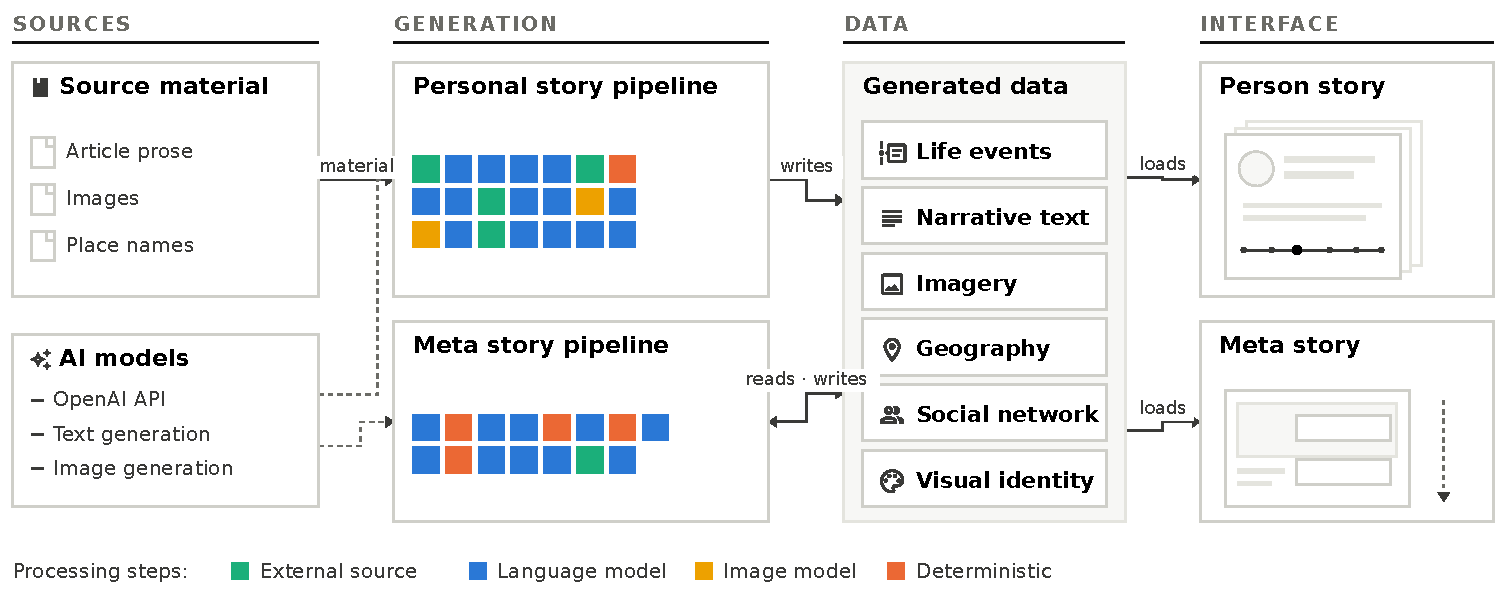
\includegraphics[width=\widewidth]{teaser.pdf}
\end{wide}
\caption{The system end to end: encyclopedic sources and model inference feed the two generation pipelines, whose data the interface reads.}\label{fig:teaser}
\end{figure}

\section{Introduction}\label{sec:introduction}

\glyphof{sources}Encyclopedic biography is a rich and well-sourced account of a life, written as continuous prose in long-form articles. Reading a life in that order is natural, but it keeps other points of access in the background and does not support more casual browsing. Such browsing would be supported by the biography's temporal, geographic, and relational structure: the phases of a life, its movements, the people who recur in it. That structure runs through the whole text without being tangible for the reader.

Life Data Stories makes that structure explicit and explorable. It derives from the source prose a set of discrete \glyphof{events}events and the documented \glyphof{network}relationships that recur across them. Each event has a resolved date, a \glyphof{places}place, the people involved, and the \glyphof{imagery}illustrations available for it. It groups those events into the phases of a life and presents the result simultaneously as narrative text, as a chronology, as a geography, and as a social network. The \glyphof{narrative}text that describes those events and the \glyphof{identity}visual identity the story is presented in are generated with them. The same derivation applied across several biographies yields a meta story, one continuous document that integrates a timeline with a lane per life, a map, and a social network merged from the biographies.

Segel and Heer [\hyperref[ref:1]{1}], surveying how data and visualization are used to tell stories, place such a presentation on a spectrum between the author-driven, in which a fixed order carries the message, and the reader-driven, in which the audience decides what to look at. A story in Life Data Stories is author-driven at first glance and reader-driven in its depth. The sequence is fixed when the story is generated and can be followed to the end. Alternative exploration affordances are available throughout, in timelines, image galleries, maps, and social network views. A meta story is linear in the same way, and at any point along it one of the lives can be entered.

BiographySampo [\hyperref[ref:2]{2}] is one of the closest precedents from the digital humanities. It extracts events, places, and relationships from national biographical dictionaries with language technology and pattern rules, links them to external registers, and offers them through faceted search, maps, timelines, and ego networks. Its tools serve biographical research, and the text of a biography stays what it was, read beside the data. VisKonnect [\hyperref[ref:3]{3}] uses encodings similar to those of Life Data Stories and connects historical figures through the events they have in common. There, only a reader's prompt retrieves the matching events from an event knowledge graph, and an event timeline, an event map, and a relationship graph are shown beside a short answer. Textual answers are generated but are only partial and stay disconnected from the visual representation. In contrast, Life Data Stories integrates text and visual representation and proposes an order through both, with exploration options alongside.

To achieve this, we heavily rely on large language models (LLMs) for interpreting the data. A biography is at first unstructured text, and giving it structure means deciding which episodes are important, which places they relate to, and which relationships matter. However, this only needs to be done once, not as part of the user interface. The system is accordingly built in two parts that connect through the data (Figure~\ref{fig:teaser}). Generation runs offline as preprocessing and interleaves model calls with deterministic transformation, so a step that researches or reviews material is surrounded by steps that resolve, cluster, merge, and validate what the model returned. It produces a set of documents, data, and images describing one life or one theme. The interface loads those files and renders them as a matter of presentation alone in a single-page web application.

\section{Data model}\label{sec:data-model}

The data that connects generation and interface is a semi-structured representation of a biography and the central abstraction of the system. For a single life it holds several structured perspectives: the \hyperref[concept:events]{\glyphof{events}events} that mark the turning points of a life, the \hyperref[concept:narrative]{\glyphof{narrative}text} that describes them, the \hyperref[concept:imagery]{\glyphof{imagery}pictures} that illustrate them, and the \hyperref[concept:places]{\glyphof{places}geography} connected to them. While these parts are relatively straightforward derivatives of the textual biographical source, two further perspectives are more interpretive: the \hyperref[concept:network]{\glyphof{network}social network} around the subject, which the text rarely describes explicitly, and the \hyperref[concept:identity]{\glyphof{identity}visual identity} the story is presented in, which gives it a recognizable look.

\begin{legend}
\glyphof{events} Life events\label{concept:events} & Dated episodes grouped into phases. \\
\glyphof{narrative} Narrative text\label{concept:narrative} & Prose describing each event and framing the story. \\
\glyphof{imagery} Imagery\label{concept:imagery} & Licensed pictures matched to events. \\
\glyphof{places} Geography\label{concept:places} & Historical place names on a modern map. \\
\glyphof{network} Social network\label{concept:network} & Typed and weighted relationships between the persons involved. \\
\glyphof{identity} Visual identity\label{concept:identity} & A palette, typography, and background pattern per story. \\
\end{legend}

A meta story refers to the data of the lives it connects and adds perspectives of its own. It names its cast of subjects and groups them into subtopics. Its chapters cut across those lives into shared periods, and each chapter references \hyperref[concept:events]{\glyphof{events}events} that stay in the subjects' own data, annotated with what each one contributes to it. The subjects' ego networks are merged into one \hyperref[concept:network]{\glyphof{network}social network}, and the \hyperref[concept:places]{\glyphof{places}geography} of all of those lives is clustered into the places important to the theme. The \hyperref[concept:narrative]{\glyphof{narrative}text} is written for the theme, and the \hyperref[concept:imagery]{\glyphof{imagery}pictures} that illustrate it are selected from the events of the individual stories. Like a life, a theme is presented in an \hyperref[concept:identity]{\glyphof{identity}visual identity} of its own.

\section{Generation}\label{sec:generation}

We split the generation of this data into two stages. The first stage, the personal story pipeline, reads an encyclopedia article and writes the data of an individual biography. The second stage, the meta story pipeline, reads the data of several individuals and writes a meta story connecting them. Both pipelines run offline as Python command-line scripts, invoked for one life or one theme at a time. A run writes the data the previous section described as JSON documents. Each step within a run reads the documents earlier steps wrote, writes its own back to disk, and is one of four kinds.

\begin{legend}
\swatch{kindexternal} External source & Fetches data from public sources. \\
\swatch{kindai} Language model & Sends a prompt to a language model and parses the structured result. \\
\swatch{kinddeterministic} Deterministic & Runs plain code to aggregate or check results through heuristics. \\
\swatch{kindimage} Image model & Generates or edits an image. \\
\end{legend}

Both pipelines follow the same pattern: material is derived bottom-up and revised top-down. Both end in translation, where the English document is written first and each document is then translated into every other supported language (currently: German).

\subsection{Personal story pipeline}\label{sec:personal-story-pipeline}

The personal story pipeline derives data for one biography, from an \glyphof{sources}encyclopedia article to the data needed for an illustrated and individually styled story. The chart (Figure~\ref{fig:pipeline-person}) bands its steps into seven phases: the sources are gathered; the events are proposed, researched, and geocoded; their pictures are found; the story is given a style and generated pictures; the social network is derived and both datasets are reviewed; a depth layer of background reports is written; and localization closes the run.

\begin{figure}[tp]
\centering
\pipelinechart{pipeline-person.pdf}
\caption{Personal story pipeline as a dependency graph. A shaded band gathers the steps of one phase.}\label{fig:pipeline-person}
\end{figure}

\emph{Sources}. An \stepref{kindexternal}{acquisition} step loads the subject's Wikipedia article and linked article titles. An AI-based \stepref{kindai}{selection} call selects the most relevant titles before their full texts are fetched. The fetched articles and Commons image metadata are cached for reuse by later steps and reruns.

\emph{Events}. The events and the main narrative are derived from that material. The first AI-based call \stepref{kindai}{proposes} twelve to sixteen events with titles, dates, descriptions, a classification, and a weight, and groups them into three to six chapters. A second call per event then \stepref{kindai}{researches} each event in detail against the relevant articles: the historic and modern name of its place, the people involved, a semantic icon, and image searches that would illustrate it. \stepref{kindexternal}{Geocoding} looks up exact coordinates for the places by their modern names.

\emph{Images}. A \stepref{kindai}{planning} step generates queries for images relating to the person's name and the subjects of the events, while the per-event searches name specific objects such as a building or a document. The \stepref{kindexternal}{search queries} are then executed against Wikimedia Commons and Openverse, and the candidates are \stepref{kinddeterministic}{scored} in code on resolution, file size, and filename before an AI-based \stepref{kindai}{matching} call assigns pictures to events, writes captions with attribution, and picks a reference portrait. Since the matching call judges by metadata only, a \stepref{kindai}{vision} call checks whether the chosen portrait, which we consider the most central visual representation, actually depicts the subject.

\emph{Presentation}. A \stepref{kindai}{color and type} system is derived from the subject's own work. The step is shown the events of the life that depict something---a building, a first edition, a manuscript, an instrument---together with the captions of the pictures the story carries, and it returns the palette with a sentence naming what that palette was read off. Selecting the events for what they show rather than for their place in the chronology is what makes the derivation possible: an opening run of births and schooldays is the same for every subject and supports no palette at all. The style is checked through rule-based heuristics regarding tile, font, and contrasts, and regenerated if necessary. Considering the style (especially the color palette), illustrations are generated: the reference portrait is \stepref{kindimage}{style-transferred} toward one master style shared by all subjects, each chapter is turned into an abstract \stepref{kindai}{visual concept} in one call over all chapters, and each concept is \stepref{kindimage}{drawn} in the same style.

\emph{Network and review}. The \stepref{kindai}{ego network} is derived independently of the style, as typed, weighted, and described relationships. A \stepref{kindai}{review} pass over the events and the network refines descriptions but applies only high-confidence changes. Reading the slides in order, it potentially rewrites descriptions that rely on names not yet introduced or repeat the previous slide.

\emph{Depth}. A \stepref{kindai}{background report} of a few paragraphs---explaining details of an event or the background of a key concept relevant to the event (e.g., an invention)---is written after the review for the most important events, roughly one event per chapter, and only where the sources say something around the event itself---an event they record in half a sentence gets no report, and the story then offers no way down there. A \stepref{kindai}{critic} call reads the illustrations found for it against the report, filtering out images that do not fully match the scope of the respective topic.

\emph{Localization}. To be able to provide multiple language options, a \stepref{kindexternal}{lookup} collects the target language's names of the subject, the people, and the places from the linked articles. A \stepref{kindai}{glossary} call fixes once per subject how every name is rendered, since cross-references between the translated documents are matched on exact names. The \stepref{kindai}{translation} merges the translated fields over a copy of the English document, so that dates, coordinates, URLs, and identifiers stay unchanged.

\subsection{Meta story pipeline}\label{sec:meta-story-pipeline}

The meta story generation (Figure~\ref{fig:pipeline-meta}) concerns a theme that connects multiple lives (e.g., an area of science, art, or political development) and builds upon the output of the personal pipelines. The story is planned and its events collected and curated against the theme. Moreover, the social network and the map are derived independently of each other. Then, a composition step joins the branches into one story and gives it a visual identity. Again, localization closes the run.

\begin{figure}[tp]
\centering
\pipelinechart{pipeline-meta.pdf}
\caption{Meta story pipeline as a dependency graph. A shaded band gathers the steps of one phase.}\label{fig:pipeline-meta}
\end{figure}

\emph{Planning}. An AI \stepref{kindai}{planning} call reads a summary of every subject and decides whom to involve from the list of available personal stories. It groups the selected people into two to four subtopics, proposes three to six chapters as named eras with estimated date ranges, and drafts a description and a conclusion. \stepref{kinddeterministic}{Event collection} then gathers every dated event of the selected people in code.

\emph{Events}. A \stepref{kindai}{curation} call per batch of events judges each event against the theme and records why it belongs. The proposed chapters are then fitted to the surviving events. Each event goes to the chapter containing its year or to the nearest one, and each span snaps to its events. A \stepref{kindai}{context} call adds up to two historical events per chapter that affected the story's people or are important historic reference points.

\emph{Network}. The network construction starts from the subjects' ego networks. An initial \stepref{kinddeterministic}{merge} joins them by normalized name into one graph of the subjects and the related people who appear in two or more of their ego networks. Since each ego network was generated for one person, a \stepref{kindai}{review} call reads the merged graph against excerpts of the subjects' articles and adds ties the ego networks missed, rewords them, or deletes indirect ones, generously on a sparse graph and strictly on a dense one. \stepref{kinddeterministic}{Community detection} by greedy modularity [\hyperref[ref:4]{4}] yields the story's circles (i.e., clusters of people), which the composition may later regroup.\footnote{The detection merges the two connected communities whose union adds the most modularity until no merge adds any, the greedy optimization of Clauset et al. (without the heaps that make their version fast, as the examples here are small).} A \stepref{kindai}{narration} call writes a title and a short description per circle.

\emph{Map}. The map branch starts from the located events the chapters reference. A \stepref{kindai}{rating} call scores each of them by how important the place appears to be for the story. The scores weight the \stepref{kinddeterministic}{clustering}, which merges events only while all of them lie close together and keeps the clusters whose weights add up, ordered by date. A \stepref{kindai}{narration} call writes a title and a short description per cluster and decides which clusters the map keeps as stops, discarding groupings that merely share a city and places that would only pad the map.

\emph{Composition}. The \stepref{kindai}{composition} call assembles the story based on the previously generated materials. In one call it revises and connects the descriptions into a coherent and consistent story and decides the order of the sections and the final grouping of the circles. A \stepref{kindai}{style} call derives from its framing a color palette, background pattern, fonts, and ornamental elements.

\emph{Localization}. Each subject's name is taken from their own translated registry entry, so that a meta story calls a person what their own story calls them. The \stepref{kindai}{translation} follows the same contract as a person's data and copies event titles verbatim from the translated person data, so that chapter and slide never disagree. Its prompt asks the translator to read the whole story before rendering the images its theme rides on, to keep a picture only where the target language uses it and otherwise to say plainly what it meant, and to hold to that decision in every passage, the title included.

\subsection{AI models and prompting}\label{sec:ai-models-and-prompting}

The generation uses OpenAI's API models (gpt-5.6-luna, gpt-5.6-sol, gpt-5.6-terra, gpt-image-2.5-flare, gpt-image-2.5-sunburst). We configure the models per call site to only spend frontier intelligence and reasoning effort where needed and keep generation costs manageable (below 1 EUR per generated story). We assign the largest model to composition, the one step that reads a whole assembled story, the image models to the portrait and chapter illustration steps, and divide the remaining steps between a reasoning tier and a small one by whether a wrong answer can quietly become part of the corpus. A step uses the small model when its output is validated against existing entities, rewritten by a later step, or backed by a deterministic fallback. More advanced tasks use the reasoning tier: proposing the events of a life, selecting the people of a theme, reviewing another step's output, the glossary, and the translation, whose wording no later step checks or rewrites. Analogously, reasoning effort is differentiated between different calls.

For prompt design and context engineering, we tried to anticipate which materials a call needs and to limit the prompt to those, while still providing sufficient background. The material shared by all calls of a step is placed at the start of the prompt and the event-specific part at the end, and the request marks where the shared part ends, so that the API caches that prefix and the later calls of the step read it instead of sending it again. Without such a marker the API caches each prompt whole, and a prompt ending in its own event is one no other call can reuse. All steps that produce text a reader sees share one instruction block on writing style. It discourages typical patterns of AI-generated prose, for instance, contrasting a fact with an alternative nobody proposed. Most text responses are requested as structured output against a \href{https://docs.pydantic.dev/}{Pydantic} schema; the style generators request JSON objects and validate them in code.

\section{Interface}\label{sec:interface}

Life Data Stories' frontend is a mobile-first Svelte application that loads the data the generation pipelines produced and renders it. The layout is designed for the phone and adapts responsively to larger screens; the screenshots in this report are deliberately captured at both phone and desktop width. The landing page offers access to the two story types, which organize the data differently: a personal story follows one life in order, and a meta story follows a theme across several lives. On the landing page (Figure~\ref{fig:shot-landing}), the meta stories are displayed in a carousel at the top. Below them, the personal stories can be reached via their generated portrait, by filtering on role, by search, or by viewing a map that plots every place mentioned across the corpus. Clicking a marker there opens directly onto the event it belongs to inside a personal story. In the following, we walk through both story types in more detail. Throughout, we use the meta story \emph{Beyond the Box} and the personal story of \emph{Antoni Gaudí} as running examples.

\begin{figure}[tp]
\begin{wide}\centering
\shotframe{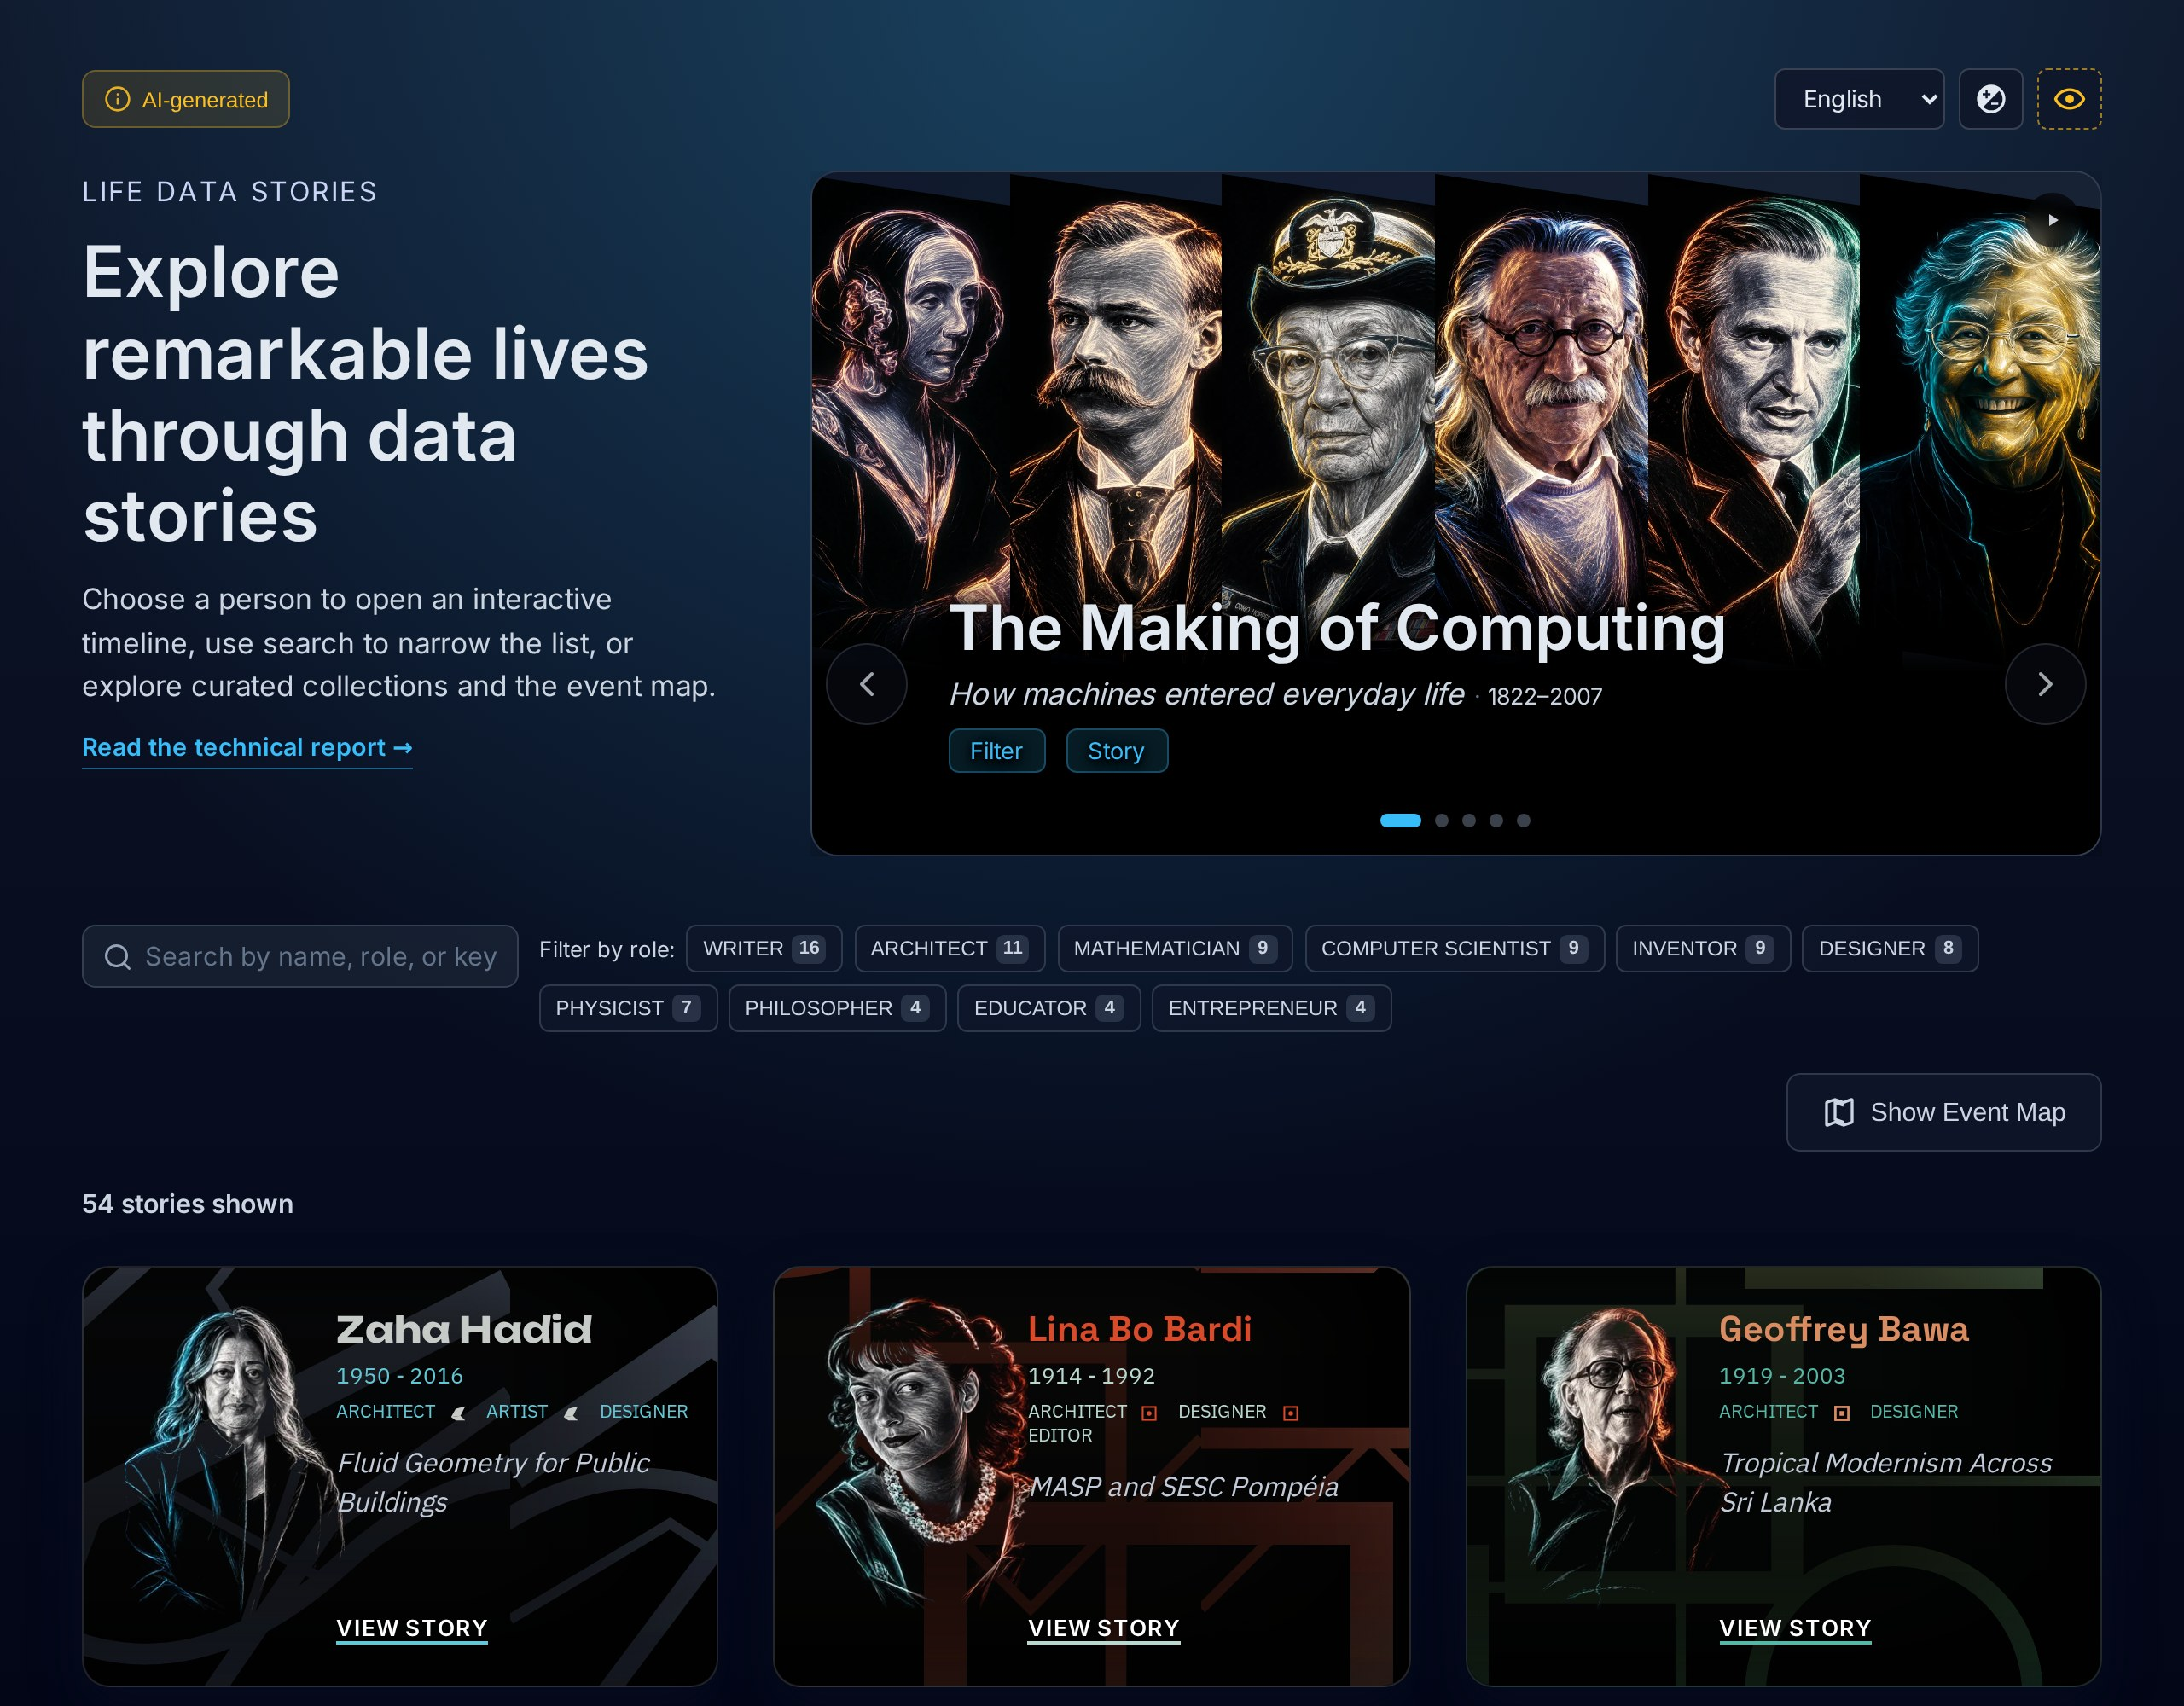
\includegraphics[width=\dimexpr\widewidth-0.8pt\relax,height=0.55\textheight,keepaspectratio]{../screenshots/landing.jpg}}
\end{wide}
\caption{The landing page: a carousel of meta stories above, the personal stories in a filterable grid below.}\label{fig:shot-landing}
\end{figure}

\subsection{The meta story}\label{sec:the-meta-story}

A meta story is structured as an opening scene, up to three sections---relating to components such as timeline, social network, and map---and a closing conclusion, followed by a grid linking to the people it covers. The whole is read from top to bottom by scrolling. \emph{Beyond the Box} follows nine architects who explored organic shapes in architecture and worked across more than a century.

\emph{Timeline.} After a short textual introduction, the vertical scrolling turns horizontal as the reader reaches the timeline visualization (Figure~\ref{fig:shot-meta-timeline-environment}). In \emph{Beyond the Box}, a timeline of nine lanes, one per architect, shows events that are marked as dots along each lane. A sequence of guiding story cards, marking chapters in the development, is pinned near the top and leads the reader through the timeline. Tapping or clicking on a dot representing an event opens a brief description of it. The surrounding card instead leads into that architect's personal story. Above the lanes is a second layer of annotations that marks the historical events affecting several lives at once, such as World War II.

\begin{figure}[tp]
\begin{wide}\centering
\shotframe{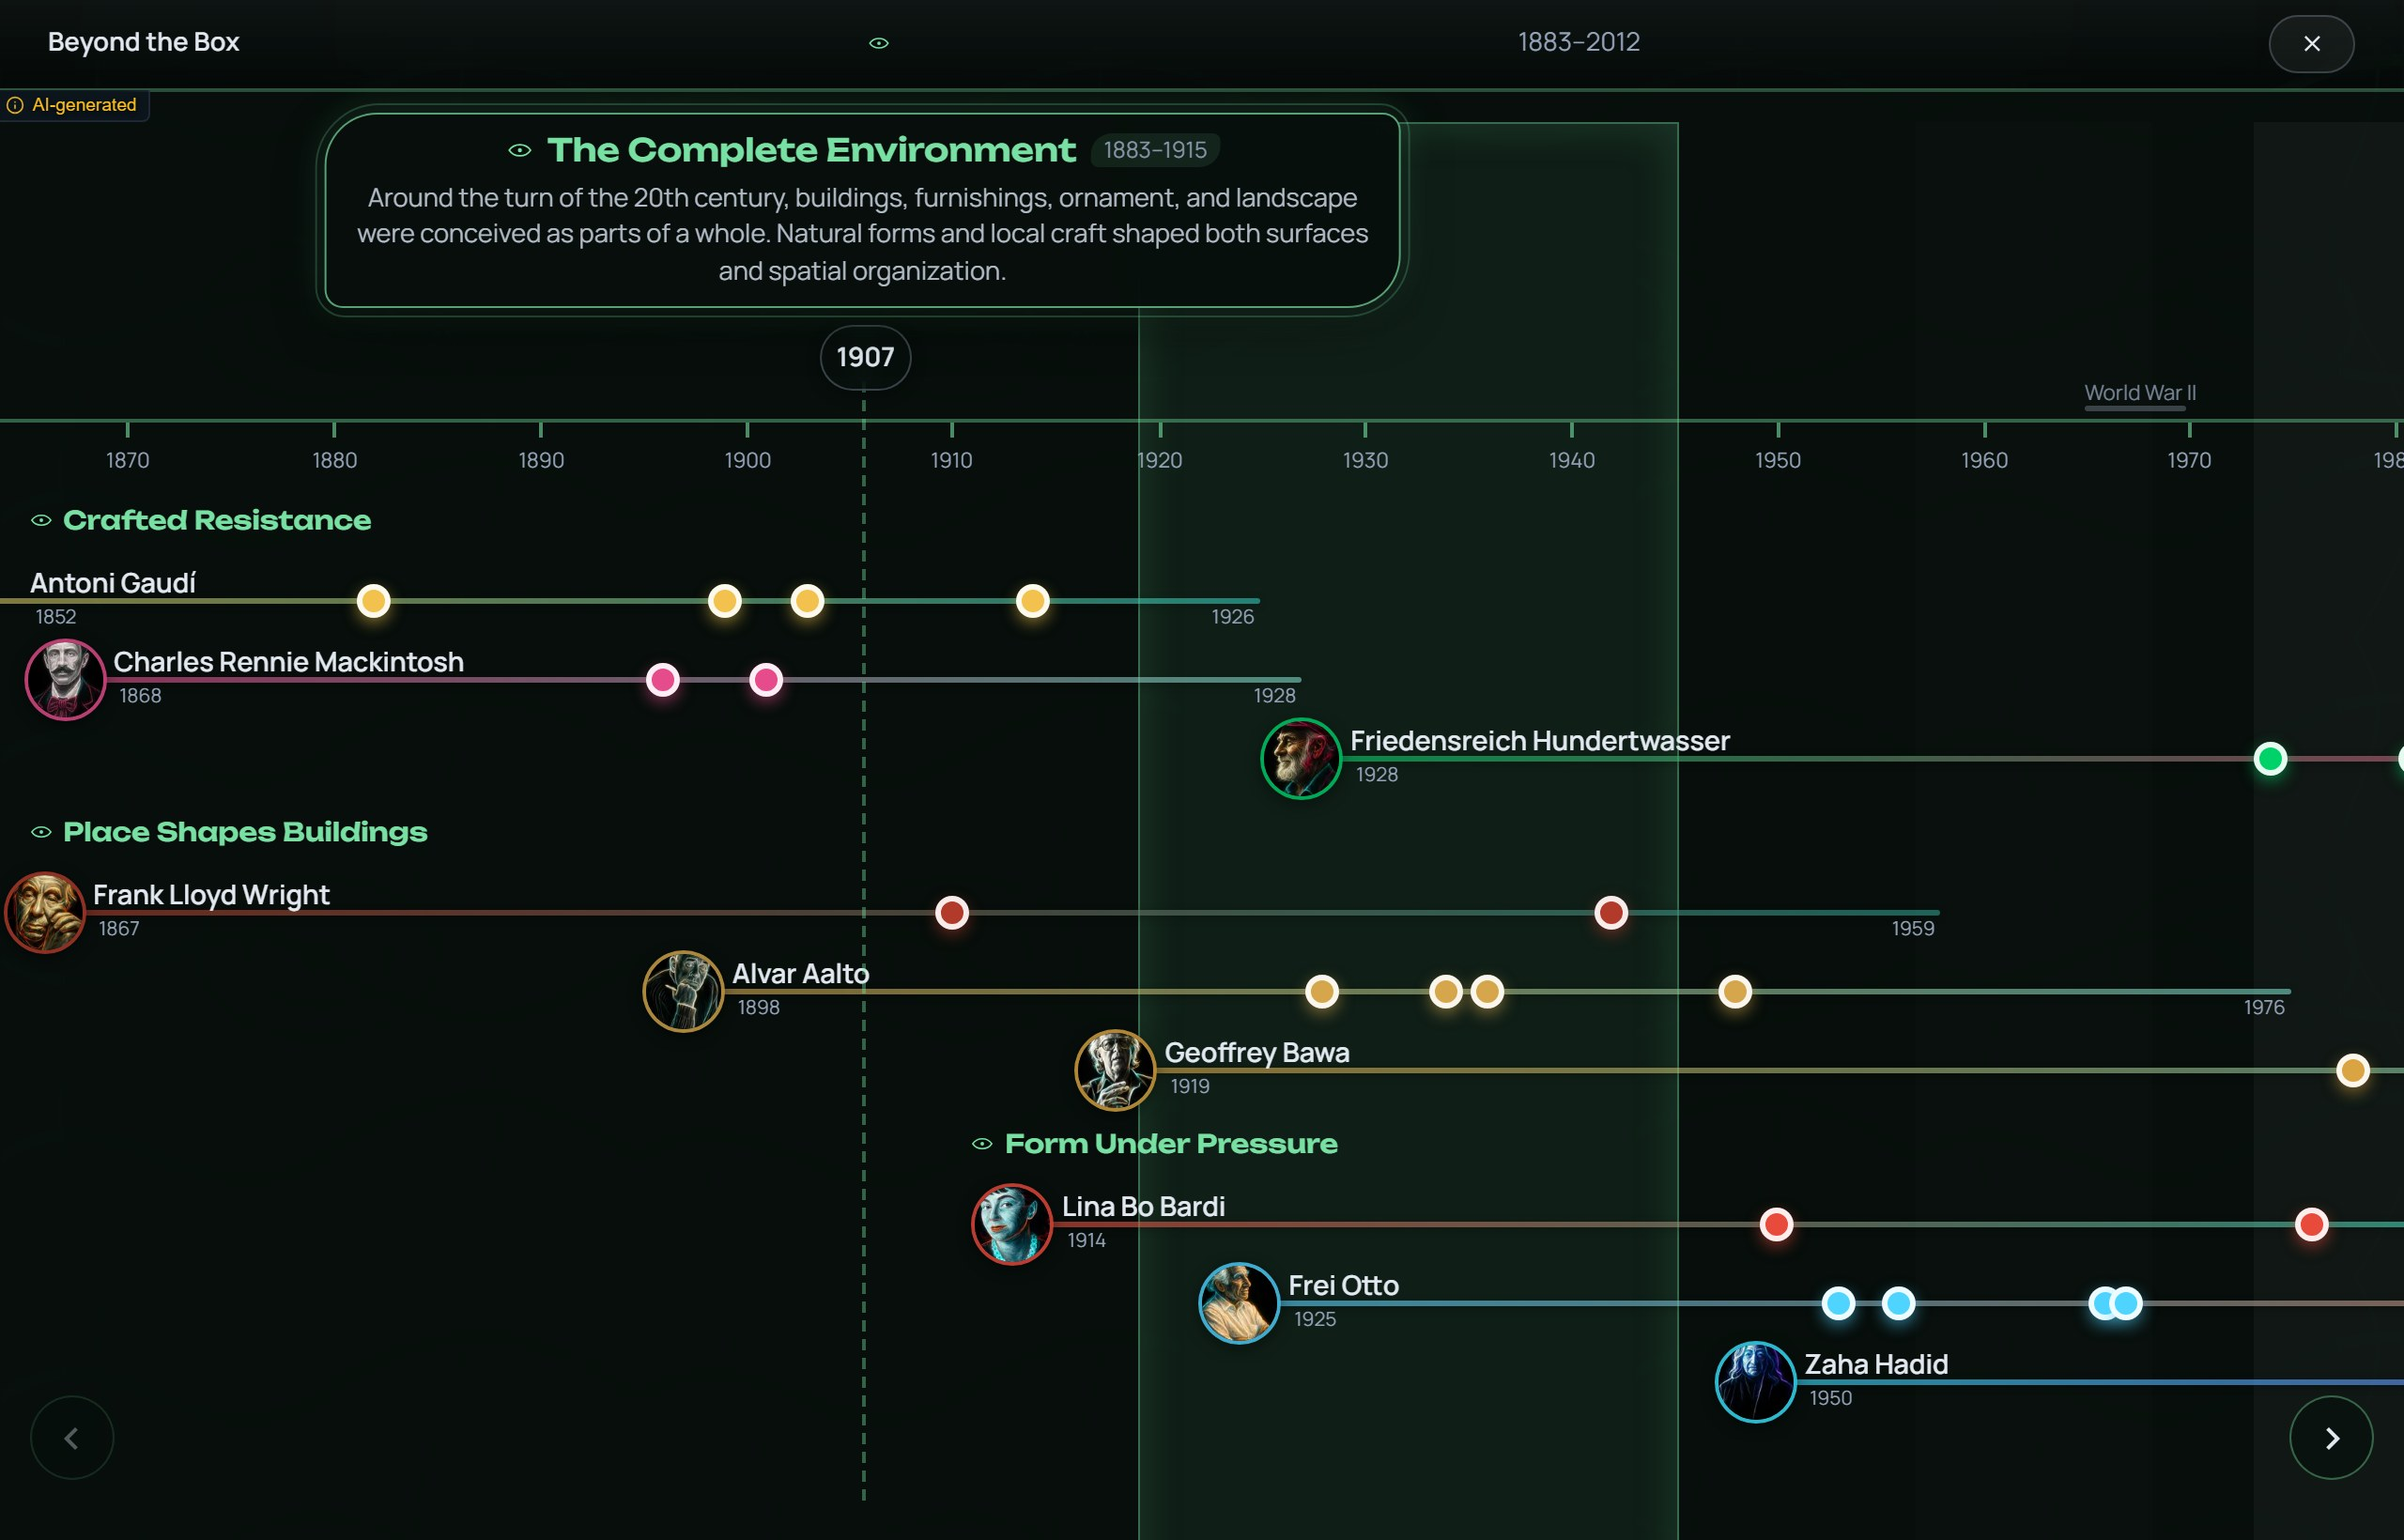
\includegraphics[width=\dimexpr\widewidth-0.8pt\relax,height=0.55\textheight,keepaspectratio]{../screenshots/meta-timeline-environment.jpg}}
\end{wide}
\caption{The timeline: one lane per architect, with a guiding story card in front naming the span currently in focus.}\label{fig:shot-meta-timeline-environment}
\end{figure}

\emph{Network.} The graph (Figure~\ref{fig:shot-meta-network}) displays the architects and the documented connections between them. Its force-directed layout is calculated in the background and finalized before it is displayed. As precomputed, the data groups people into clusters. As the reader scrolls, cards move over the graph, one per cluster, describing it, and the people and connections involved are highlighted, while the rest of the graph darkens.

\begin{figure}[tp]
\centering
\begin{minipage}[t]{0.47\linewidth}\centering
\shotframe{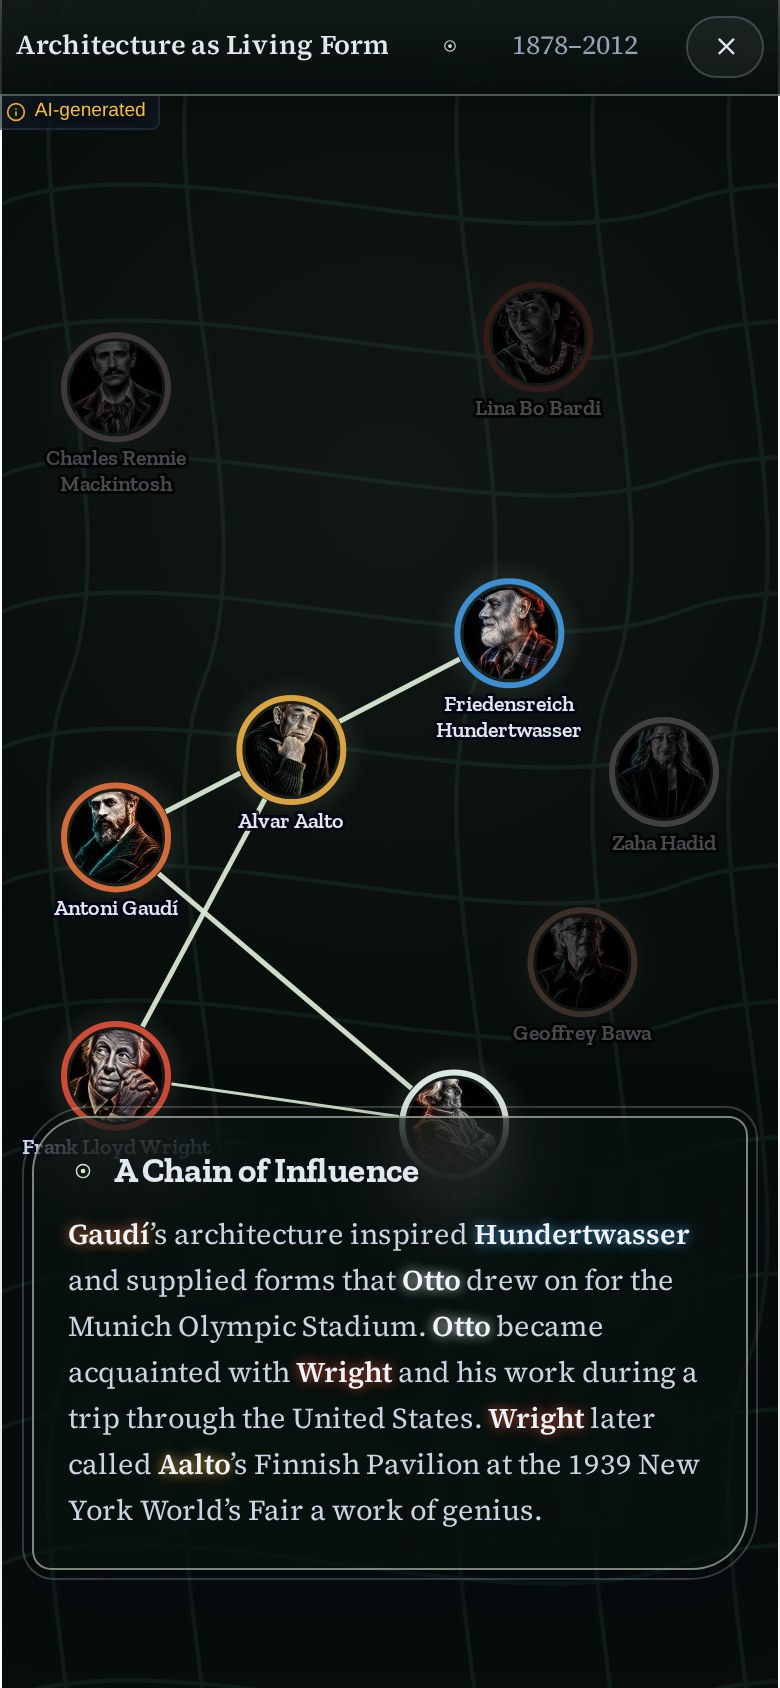
\includegraphics[width=\dimexpr\linewidth-0.8pt\relax,height=0.4\textheight,keepaspectratio]{../screenshots/meta-network.jpg}}
\caption{The network: architects as nodes, one card in front naming the cluster currently lit.}\label{fig:shot-meta-network}
\end{minipage}\hfill
\begin{minipage}[t]{0.47\linewidth}\centering
\shotframe{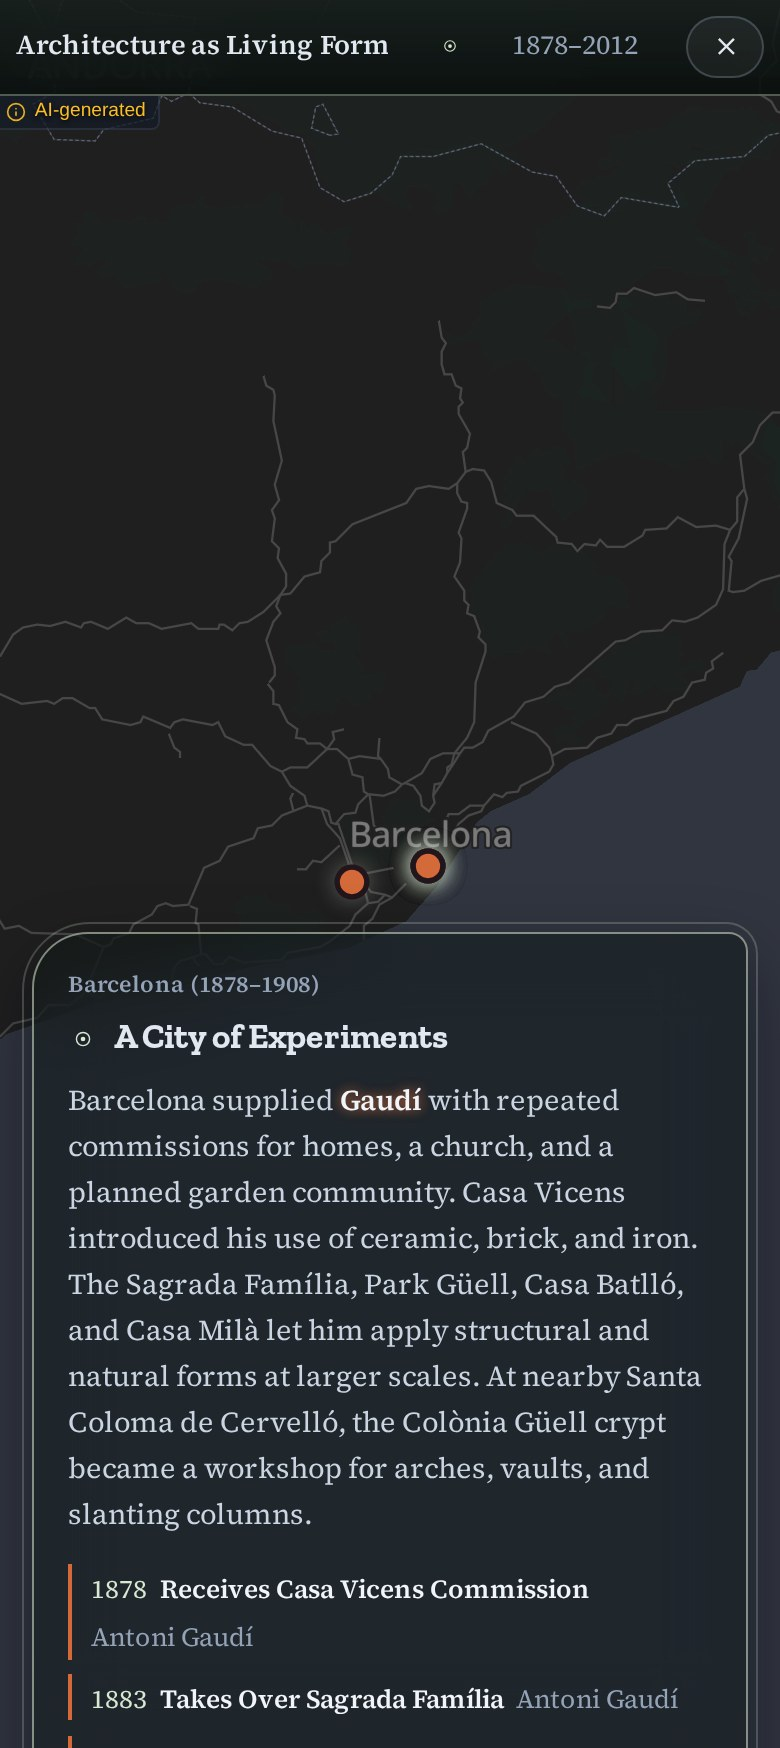
\includegraphics[width=\dimexpr\linewidth-0.8pt\relax,height=0.4\textheight,keepaspectratio]{../screenshots/meta-map.jpg}}
\caption{A location card, with the map flown in above and its linked events listed below.}\label{fig:shot-meta-map}
\end{minipage}
\end{figure}

\emph{Map.} The third section shifts the focus to the locations where the architects' work took place. A non-interactive map (Figure~\ref{fig:shot-meta-map}) fills the background behind the scrollable story cards, flying to a new location as each one scrolls into view. It zooms to a point or fits a bounding box depending on how spread out the events are. Each event listed on a card links directly to the respective personal story.

The meta story concludes with a brief summary that ties the nine lives together. Below that is a grid of tiles, one for each architect, that links out to the architects' personal stories.

\subsection{Personal story}\label{sec:personal-story}

Following that grid into Gaudí's personal story opens it at its beginning, showing the stylized portrait image and a short biographical summary. The same three encodings of time, place, and relation that a meta story spreads across sections are attached to this sequence too, just differently. The story unfolds as a horizontal sequence of slides, moved through by swiping sideways. Chapter slides, showing a headline and an illustration, structure the event slides (Figure~\ref{fig:shot-gaudi-relationship-card}) that provide the main information. Aside details of the event, an image might be blended in. For events with supporting data, a vertical axis opens further. A chevron reveals a longer background passage about the context of the event. Special events such as birth, death, publication, or migration contain further structuring elements and specialized representations.

\begin{figure}[tp]
\centering
\begin{minipage}[t]{0.31\linewidth}\centering
\shotframe{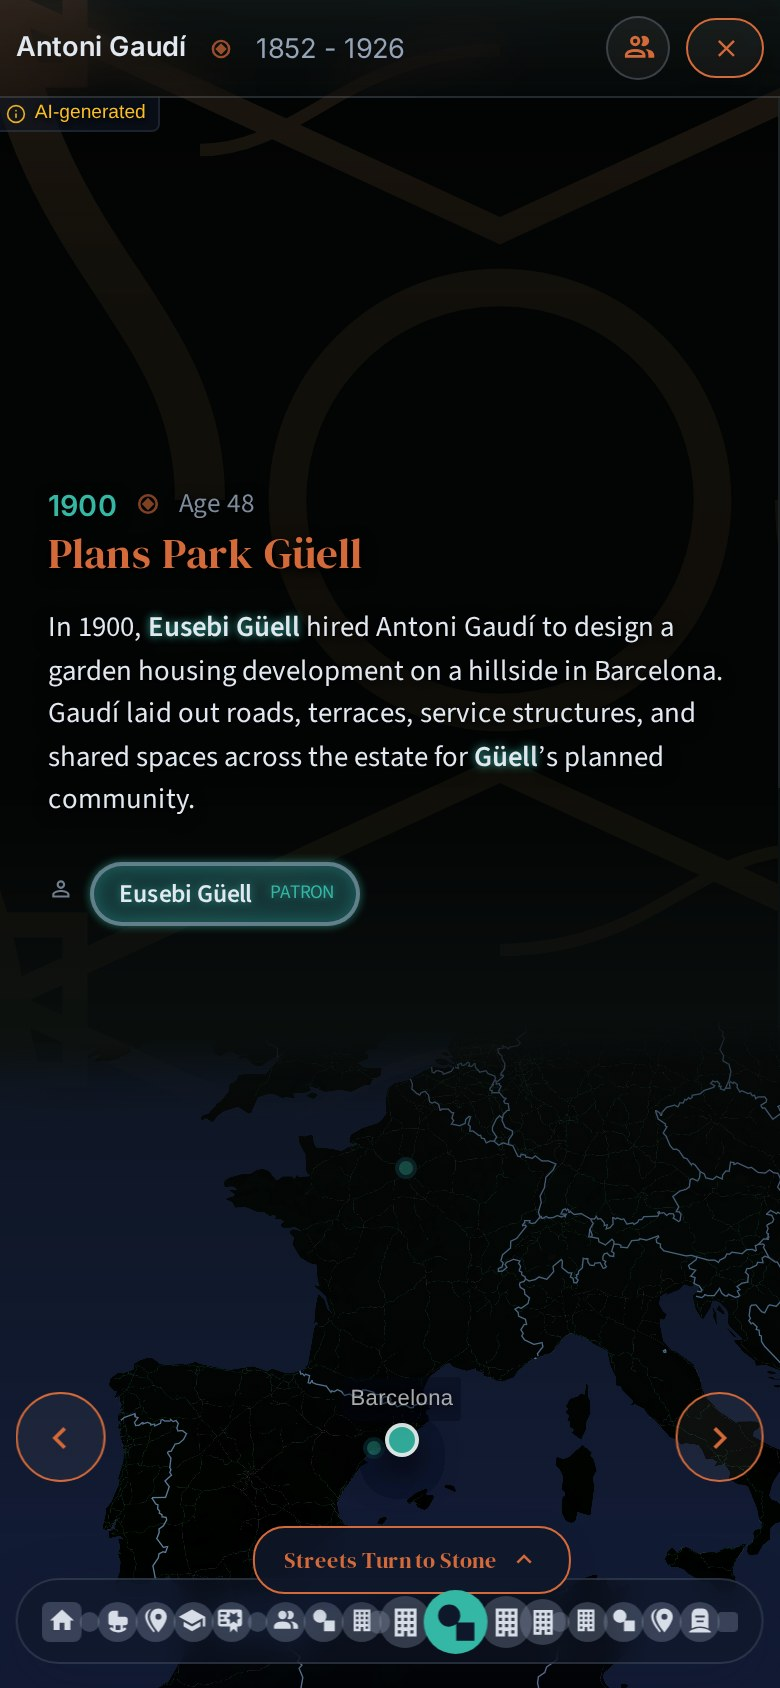
\includegraphics[width=\dimexpr\linewidth-0.8pt\relax,height=0.4\textheight,keepaspectratio]{../screenshots/gaudi-relationship-card.jpg}}
\caption{The classic format of the slide includes text in the middle, a map beneath, and an outline consisting of icons at the bottom.}\label{fig:shot-gaudi-relationship-card}
\end{minipage}\hfill
\begin{minipage}[t]{0.31\linewidth}\centering
\shotframe{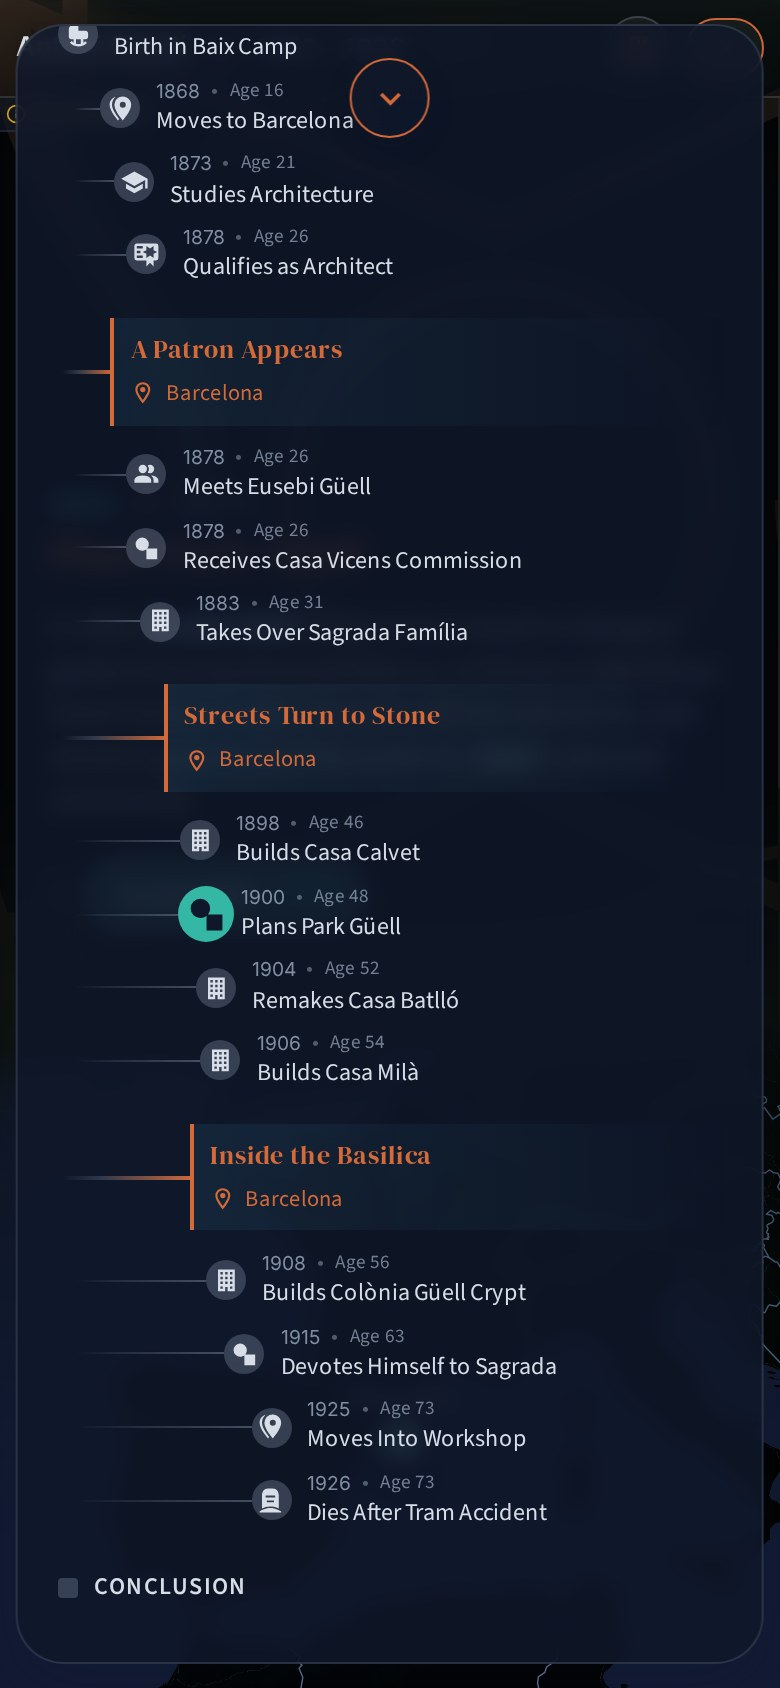
\includegraphics[width=\dimexpr\linewidth-0.8pt\relax,height=0.4\textheight,keepaspectratio]{../screenshots/gaudi-timeline.jpg}}
\caption{The expanded timeline: the life as a vertical outline of chapters and events, each entry led in by a line that grows with the subject's age.}\label{fig:shot-gaudi-timeline}
\end{minipage}\hfill
\begin{minipage}[t]{0.31\linewidth}\centering
\shotframe{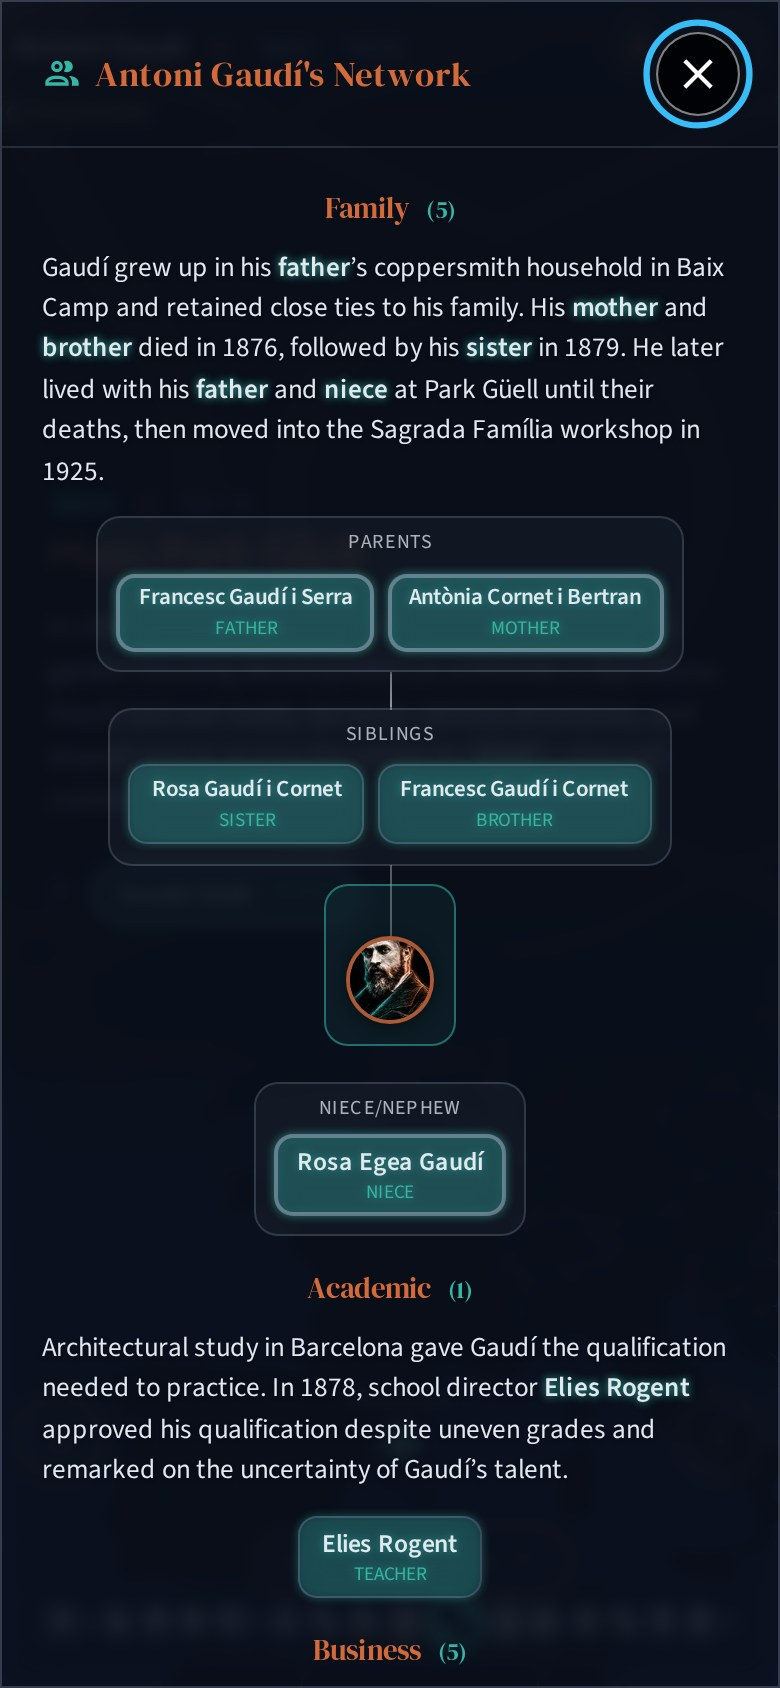
\includegraphics[width=\dimexpr\linewidth-0.8pt\relax,height=0.4\textheight,keepaspectratio]{../screenshots/gaudi-network.jpg}}
\caption{The network view of a personal story: relationships by category, the family laid out as generations around the subject and the other categories in boxes labeled by role.}\label{fig:shot-gaudi-network}
\end{minipage}
\end{figure}

\emph{Timeline.} As an explicit representation of time, a row along the bottom serves as both a progress marker and an outline. Each event is represented by an icon that reflects its type, while each chapter is represented by a plain marker. Tapping the row unfolds it into a full-screen outline of the life (Figure~\ref{fig:shot-gaudi-timeline}), the icons traveling from their places in the row to their entries in the list. The outline runs from the overview to the conclusion, with each chapter as a heading that names its main location and each event beneath its chapter with year, the subject's age, and title. Each entry is set in from the left in proportion to the subject's age at that point, so the pace of the life stays visible where the list is dense. Tapping an entry closes the outline and moves the story to that slide.

\emph{Map.} Fixed in the same position on the screen, the map receives a marker each time an event mentions a place. Hence, by the end of the story, the map shows everywhere the subject worked and lived. In the example, the event's main marker is on Barcelona, while a secondary marker is visible on Paris and a faded smaller one close to Barcelona.

\emph{Network.} When an event slide mentions another person, that person's name appears beside the text with their role, as here for Eusebi Güell, tagged as patron. Tapping the tag opens a card describing the relationship on its own terms. From this card, or the button at the top of the screen, readers can access Gaudí's full network (Figure~\ref{fig:shot-gaudi-network}). It is organized by relationship category, family first and then the others in alphabetical order, professional, religious, and social in Gaudí's case. Each category has a count and a short passage that introduces its people, with the names and roles it mentions highlighted, and lays them out as chips grouped by role: the family as generations around the subject, joined by lines, and the other categories in boxes labeled by role, such as collaborator or patron. Tapping a chip opens the description and strength of that relationship.

\section{Discussion and conclusion}\label{sec:discussion-and-conclusion}

This report has introduced the implementation of Life Data Stories, an approach for transforming unstructured biographical text into structured stories about individual lives and the themes that connect them. It defines the main structuring elements of these stories: \glyphof{events}life events, \glyphof{narrative}narrative text, \glyphof{imagery}imagery, \glyphof{places}geography, and \glyphof{network}social network views, which together provide affordances for interactive exploration. The stories follow one consistently styled theme while their \glyphof{identity}visual identity adapts to the specific person, which gives each story a recognizable visual profile. The approach relies on AI-based extraction to derive the underlying structured data. This step runs as preprocessing, so the presentation layer stays independent of further AI calls. At the same time, the resulting stories remain highly interactive through the extracted data layers and the connections between them.

While this report provides implementation details and a basic scientific contextualization, a broader scientific discussion is beyond its scope. Such a discussion would consider related scientific explorations in similar directions and the corresponding empirical work in more detail. Likewise, an evaluation of the approach has not been part of the present focus and remains future work. As the approach targets a broad audience, feedback from users within this audience will be an important part of such an evaluation. Beyond usability and the perceived value of the approach, it should investigate to what extent users accept AI-based transformations of biographical sources and what expectations they have regarding such transformations.

\section{References}\label{sec:references}

\begin{reflist}
\item\label{ref:1} E. Segel and J. Heer, ``Narrative Visualization: Telling Stories with Data,'' \emph{IEEE Transactions on Visualization and Computer Graphics}\refdetail{, vol. 16, no. 6, pp. 1139--1148, 2010, }\refdetail{doi: }\href{https://doi.org/10.1109/TVCG.2010.179}{\refdoi{10.\allowbreak{}1109/\allowbreak{}TVCG.\allowbreak{}2010.\allowbreak{}179}}\refdetail{.}
\item\label{ref:2} E. Hyvönen, P. Leskinen, M. Tamper, H. Rantala, E. Ikkala, J. Tuominen, and K. Keravuori, ``BiographySampo -- Publishing and Enriching Biographies on the Semantic Web for Digital Humanities Research,'' \refdetail{in }\emph{The Semantic Web (ESWC 2019)}\refdetail{, vol. 11503, pp. 574--589, }\refdetail{doi: }\href{https://doi.org/10.1007/978-3-030-21348-0_37}{\refdoi{10.\allowbreak{}1007/\allowbreak{}978-\allowbreak{}3-\allowbreak{}030-\allowbreak{}21348-\allowbreak{}0\_\allowbreak{}37}}\refdetail{.}
\item\label{ref:3} S. Latif, S. Agarwal, S. Gottschalk, C. Chrosch, F. Feit, J. Jahn, T. Braun, Y. C. Tchenko, E. Demidova, and F. Beck, ``Visually Connecting Historical Figures Through Event Knowledge Graphs,'' \refdetail{in }\emph{2021 IEEE Visualization Conference (VIS)}\refdetail{, pp. 156--160, }\refdetail{doi: }\href{https://doi.org/10.1109/VIS49827.2021.9623313}{\refdoi{10.\allowbreak{}1109/\allowbreak{}VIS49827.\allowbreak{}2021.\allowbreak{}9623313}}\refdetail{.}
\item\label{ref:4} A. Clauset, M. E. J. Newman, and C. Moore, ``Finding Community Structure in Very Large Networks,'' \emph{Physical Review E}\refdetail{, vol. 70, no. 6, Art. no. 066111, 2004, }\refdetail{doi: }\href{https://doi.org/10.1103/PhysRevE.70.066111}{\refdoi{10.\allowbreak{}1103/\allowbreak{}PhysRevE.\allowbreak{}70.\allowbreak{}066111}}\refdetail{.}
\end{reflist}

\clearpage
\appendix
\titleformat{\section}{\Large\bfseries}{Appendix~\thesection}{0.8em}{}[{\color{rulestrong}\titlerule}]
\section{Step details}\label{sec:appendix-steps}

The steps of the personal story pipeline (Figure~\ref{fig:pipeline-person}) and the meta story pipeline (Figure~\ref{fig:pipeline-meta}), one per row: description, input, output, model with reasoning effort, and calls per run.

\begin{steptable}{@{}S{0.14}S{0.36}S{0.13}S{0.13}S{0.16}S{0.08}@{}}
\tabtoprule
\textbf{Step} & \textbf{Description} & \textbf{Input} & \textbf{Output} & \textbf{Model (effort)} & \textbf{\#Calls} \\
\tabheadrule
\endhead
\multicolumn{6}{@{}p{\dimexpr\widewidth-2\tabcolsep\relax}@{}}{\lanerow{Personal story}} \\*
\stepref{kindexternal}{\textbf{Fetch Wikipedia}} & Collects the subject article, related candidates, and Commons image metadata as shared reporting material. Caches the material under a stable subject identity so later steps and reruns reuse the same source set. & A subject or article URL & Cached Wikipedia material &  & 1 \\
\tabrowrule
\stepref{kindai}{\textbf{Select articles}} & Ranks linked articles by their value for a life story. It keeps people, personal events, and individual works, so later research spends its context on relationships and moments that shape the subject's biography. & The article and outgoing link candidates & Ranked articles for biographical context & \code{gpt{-}\allowbreak{}5.6{-}\allowbreak{}luna (none)} & 1 \\
\tabrowrule
\stepref{kindai}{\textbf{Propose events}} & Selects the events that carry a life and orders them into chapters. It compares moments across the whole record, so importance and chapter breaks reflect the shape of the life rather than isolated facts. Leaves a dated narrative spine and a conclusion about work that persists. & The article and selected related articles & A chaptered life timeline and conclusion & \code{gpt{-}\allowbreak{}5.6{-}\allowbreak{}terra (medium)} & 1 \\
\tabrowrule
\stepref{kindai}{\textbf{Research events}} & Researches each proposed event against the subject's article and event-specific related material. It expands the event into grounded prose, places, people, sources, annotations, an icon, and picture-search terms; failed calls leave the event unresolved so the story continues. & An event skeleton and Wikipedia material & Researched details for each event & \code{gpt{-}\allowbreak{}5.6{-}\allowbreak{}luna (low)} & 12--16 (one per event) \\
\tabrowrule
\stepref{kindai}{\textbf{Plan image searches}} & Plans image searches across the life, reserving person searches for the portrait and tying the rest to event subjects. It avoids commemorative objects, which can displace images of the person's work and surroundings. & The event skeletons & Search strings for life images & \code{gpt{-}\allowbreak{}5.6{-}\allowbreak{}luna (none)} & 1 \\
\tabrowrule
\stepref{kindexternal}{\textbf{Search image sources}} & Searches Commons and Openverse for the planned image searches, then leaves one candidate record per picture. It searches event-specific names in Commons first so a matching picture keeps its event link when sources return the same URL. & The planned and event image searches & Deduplicated image candidates linked to events &  & 1 \\
\tabrowrule
\stepref{kinddeterministic}{\textbf{Rank candidates}} & Scores the shared image pool and retains a ranked set of viable candidates for event matching. It penalizes commemorative plaques and graves so polished modern memorial photos do not displace period images on technical quality alone. & Every image hit the queries returned & Ranked image candidates for event matching &  & 1 \\
\tabrowrule
\stepref{kindai}{\textbf{Match images}} & Selects a reference portrait and assigns only images with a direct link to life events. It leaves weak candidates unused, because a searched-for event or a shared place and date does not make an image evidence for that event. & The ranked image candidates & A portrait and event images & \code{gpt{-}\allowbreak{}5.6{-}\allowbreak{}luna (low)} & 1 \\
\tabrowrule
\stepref{kindai}{\textbf{Verify portrait}} & Checks the chosen portrait against the person in the story by inspecting the image itself. It removes a rejected portrait, while a failed check preserves the pick so a service error cannot discard it before the life events and person registry are written. & The portrait pick & Life events and person registry & \code{gpt{-}\allowbreak{}5.6{-}\allowbreak{}terra (none)} & 0-1 \\
\tabrowrule
\stepref{kindexternal}{\textbf{Geocode places}} & Adds map coordinates to places in life events. It prefers the researcher's modern name so renamed historic places retain a current map location. & Historic and modern place names & Coordinates on life events &  & 1 \\
\tabrowrule
\stepref{kindai}{\textbf{Design interface style}} & Derives a dark color, type, and geometric pattern system from the finished events and their depicted works. It requires the palette rationale to name the material evidence behind the colors. A contrast check rejects illegible palettes and sends the reason back for one revision. & The finished life events & An evidence-based interface style & \code{gpt{-}\allowbreak{}5.6{-}\allowbreak{}luna (low)} & 1 \\
\tabrowrule
\stepref{kindai}{\textbf{Build ego network}} & Builds the subject's network from finished life events and Wikipedia material. It keeps only documented direct ties between named people, so later story work can join personal, professional, and political relationships without treating institutions as people. & Finished life events and Wikipedia material & A documented network of personal ties & \code{gpt{-}\allowbreak{}5.6{-}\allowbreak{}terra (medium)} & 1 \\
\tabrowrule
\stepref{kindimage}{\textbf{Draw portrait}} & Redraws each licensed reference portrait in the story's shared line style and colors, then records the finished portrait for the person and their life events. It separates identity from rendering by using the source portrait for likeness and a master portrait for technique. & The person registry and interface style & A styled portrait and updated person record & \code{gpt{-}\allowbreak{}image{-}\allowbreak{}2.5{-}\allowbreak{}sunburst} & 1 \\
\tabrowrule
\stepref{kindai}{\textbf{Draft chapter concepts}} & Develops an abstract opening image for each chapter from the verified life events. It considers all chapters together so their metaphors stay distinct, while avoiding depictions of the person, places, or historical events themselves. & The finished life events & An abstract visual concept per chapter & \code{gpt{-}\allowbreak{}5.6{-}\allowbreak{}terra (medium)} & 1 \\
\tabrowrule
\stepref{kindimage}{\textbf{Draw chapter art}} & Draws one abstract chapter image from each chapter concept. It carries the portrait style and story colors into the chapter images, while the concept supplies the subject; it also removes images left by renamed or deleted chapters. & Chapter concepts, story colors, and style & An illustration for each current chapter & \code{gpt{-}\allowbreak{}image{-}\allowbreak{}2.5{-}\allowbreak{}flare} & one per chapter \\
\tabrowrule
\stepref{kindai}{\textbf{Review data}} & Reviews the life events and ego network as one biography, checking facts against the supplied source material and tracing continuity across the event sequence. Leaves proposed corrections for both artifacts; the pipeline applies only changes the critic rates with high confidence. & The life events, network, and Wikipedia material & Reviewed life events and ego network & \code{gpt{-}\allowbreak{}5.6{-}\allowbreak{}terra} & 1 \\
\tabrowrule
\stepref{kindexternal}{\textbf{Collect name evidence}} & Gathers the target-language article and linked names that anchor later translations in published usage. It retries unresolved comma-qualified places under their leading name, while keeping the qualifier available for translation. & Reviewed names, life events, and ego network & Target-language article and name evidence &  & 1 \\
\tabrowrule
\stepref{kindai}{\textbf{Build name glossary}} & Decides the target-language form of each person name before translation begins. It writes one shared glossary for the life events, network, and registry, so exact-name links remain stable across documents. Source evidence takes priority when it identifies the same person. & Name evidence and person names & A shared localized name glossary & \code{gpt{-}\allowbreak{}5.6{-}\allowbreak{}terra (low)} & 1 \\
\tabrowrule
\stepref{kindai}{\textbf{Translate data}} & Translates the narrative text across the person's events, network, registry, and reports. It applies the name glossary and target-language evidence, while the merge keeps dates, coordinates, links, and identifiers from the English record. & The person record, reports, and name mapping & Localized person data & \code{gpt{-}\allowbreak{}5.6{-}\allowbreak{}terra (medium)} & 1 \\
\tabrowrule
\stepref{kindai}{\textbf{Write background reports}} & Writes event-specific background only when the reviewed articles add context beyond the event itself. It drops stale reports that fail this test and refreshes each event's citations from the articles it was given, including events left without a report. & The reviewed events, articles, and story outline & Background reports and event-specific citations & \code{gpt{-}\allowbreak{}5.6{-}\allowbreak{}terra (low)} & one per deep event --- roughly one per chapter \\
\tabrowrule
\stepref{kindai}{\textbf{Illustrate reports}} & Reviews Commons results against each report and keeps only pictures that directly depict named things. It reads filenames with captions because captions often describe the upload, and code admits only one result from each search. & The report, its searches, and life events & Report illustrations for each event & \code{gpt{-}\allowbreak{}5.6{-}\allowbreak{}terra (medium)} & 1 per report illustrated \\
\tabrowrule
\multicolumn{6}{@{}p{\dimexpr\widewidth-2\tabcolsep\relax}@{}}{\lanerow{Meta story}} \\*
\stepref{kindai}{\textbf{Plan story}} & Selects the people who belong in the theme and writes the story's title, introduction, subtopics, chapters, conclusion, and gaps in the registry. It draws on each person's roles, summary, places, and event history so place-based themes rest on recorded activity as well as biography. & The person registry and life events & A themed story plan and selected people & \code{gpt{-}\allowbreak{}5.6{-}\allowbreak{}terra (medium)} & 1 \\
\tabrowrule
\stepref{kinddeterministic}{\textbf{Collect events}} & Collects every dated life event for the selected people and orders them by year. It leaves relevance and chapter placement to later steps because early chapter ranges can miss events outside their guessed bounds. & The selected people and life events & Dated events in chronological order &  & 1 \\
\tabrowrule
\stepref{kindai}{\textbf{Curate events}} & Judges each biographical event against the story's theme and keeps only landmark contributions with a lasting output. It records a short reason for every decision, leaving the chapter-fitting stage to work from the events that survive. & The unfiltered event pool & Essential events with relevance reasons & \code{gpt{-}\allowbreak{}5.6{-}\allowbreak{}luna (low)} & one per batch \\
\tabrowrule
\stepref{kindai}{\textbf{Add historical context}} & Places each chapter in the wider events that directly shaped the people it follows. It leaves chapters with a small set of dated historical landmarks, and admits that some periods need none to avoid generic background history. & The fitted chapters with their surviving events & Historical landmarks for each chapter & \code{gpt{-}\allowbreak{}5.6{-}\allowbreak{}terra (medium)} & 1 \\
\tabrowrule
\stepref{kinddeterministic}{\textbf{Merge networks}} & Combines the selected people's ego networks into one social graph. It keeps direct ties and shared acquaintances that connect multiple main people, matching names across source networks and preserving each person's account of a direct relationship. & Selected people and ego networks & A merged social network &  & 1 \\
\tabrowrule
\stepref{kindai}{\textbf{Review network}} & Reviews the merged network against the article evidence. It adds missed direct ties and removes vague or indirect ones before clustering, while using graph density to set how readily it proposes new links. & The deterministically merged graph & A reviewed network of biographical ties & \code{gpt{-}\allowbreak{}5.6{-}\allowbreak{}terra (medium)} & 1 \\
\tabrowrule
\stepref{kinddeterministic}{\textbf{Detect circles}} & Finds communities in the reviewed graph and writes each circle's main members, related people, and internal ties into the story data. It orders circles by the main members' birth years and gives each a member-based key, so narration can retain the same circles without rerunning detection. & The reviewed graph & Ordered circles with members and ties &  & 1 \\
\tabrowrule
\stepref{kindai}{\textbf{Narrate circles}} & Turns each detected circle's ties into a factual title and short account of its bonds and bridges. It keeps the circle membership with the prose, and writes nothing unless every detected circle receives an account. & The circles to narrate & A title and text per circle & \code{gpt{-}\allowbreak{}5.6{-}\allowbreak{}luna (none)} & 1 \\
\tabrowrule
\stepref{kindai}{\textbf{Rate map events}} & Rates each located event by how strongly its place carries the story's theme. The map branch uses these scores as clustering weights, while unrated events retain a neutral weight if a batch fails. & The chapters and life events & Geographic weights for map events & \code{gpt{-}\allowbreak{}5.6{-}\allowbreak{}luna (none)} & 1 \\
\tabrowrule
\stepref{kinddeterministic}{\textbf{Cluster places}} & Groups rated events into places whose members all lie within the map's distance limit. It centers each place on the more important events, keeps the strongest places with a minimum fallback, and orders them through time for the story's route. & Located events and per-event weights & Selected map stops with their events &  & 1 \\
\tabrowrule
\stepref{kindai}{\textbf{Narrate map stops}} & Turns geographic clusters into short, factual place narratives for the meta story. It also keeps only the places that carry the story's arc, so weak or accidental groupings can be pruned from the map. & The qualifying geographic clusters & Curated map stops with place narratives & \code{gpt{-}\allowbreak{}5.6{-}\allowbreak{}luna (low)} & 1 \\
\tabrowrule
\stepref{kindai}{\textbf{Compose story}} & Composes the assembled material into one story, rewriting component text in a shared voice and choosing its narrative order. It can remove map stops that do not support the throughline, then leaves a finished meta story for later styling and translation. & The narrations, source material, and person registry & A composed meta story & \code{gpt{-}\allowbreak{}5.6{-}\allowbreak{}sol} & 1 \\
\tabrowrule
\stepref{kindai}{\textbf{Design story style}} & Derives the story's dark visual identity from its framing and opening. It ties typography, color, geometric pattern, and ornamental marks to the theme, using abstract geometry to carry the period and subject across the story. & The story's framing and opening & The story's visual style & \code{gpt{-}\allowbreak{}5.6{-}\allowbreak{}luna (low)} & 1 \\
\tabrowrule
\stepref{kindexternal}{\textbf{Collect name evidence}} & Records the names that tie a meta story to its translated person stories. It uses each person's own localized title first and queries encyclopedia language links only for map places without that record. & The composed meta story and localized person data & Name evidence for people and places &  & 1 \\
\tabrowrule
\stepref{kindai}{\textbf{Translate meta story}} & Translates the meta story while preserving its links to the localized person records. It carries settled name forms and event titles into the story, and makes one consistent choice for each metaphor across titles and prose. & The meta story and localized person data & A localized meta story & \code{gpt{-}\allowbreak{}5.6{-}\allowbreak{}terra} & 1 \\
\tabbottomrule
\end{steptable}

\vspace{24pt}{\color{rulestrong}\hrule}\vspace{6pt}
\begin{minipage}{\textwidth}\sffamily\footnotesize\color{muted}
\eyebrow{Statement on AI use}\par\vspace{3pt}
This report was co-written with AI. Its text and figures were drafted and revised with language models under the authors' direction, alongside manual edits. The system the report describes was implemented through AI using agentic engineering.\par
\end{minipage}

\end{document}
